%%%%%%%%%%%%%%%%%%%%%%%%
%% Sample use of the infthesis class to prepare a thesis. This can be used as 
%% a template to produce your own thesis.
%%
%% The title, abstract and so on are taken from Martin Reddy's csthesis class
%% documentation.
%%
%% MEF, October 2002
%%%%%%%%%%%%%%%%%%%%%%%%

%%%%
%% Load the class. Put any options that you want here (see the documentation
%% for the list of options). The following are samples for each type of
%% thesis:
%%
%% Note: you can also specify any of the following options:
%%  logo: put a University of Edinburgh logo onto the title page
%%  frontabs: put the abstract onto the title page
%%  deptreport: produce a title page that fits into a Computer Science
%%      departmental cover [not sure if this actually works]
%%  singlespacing, fullspacing, doublespacing: choose line spacing
%%  oneside, twoside: specify a one-sided or two-sided thesis
%%  10pt, 11pt, 12pt: choose a font size
%%  centrechapter, leftchapter, rightchapter: alignment of chapter headings
%%  sansheadings, normalheadings: headings and captions in sans-serif
%%      (default) or in the same font as the rest of the thesis
%%  [no]listsintoc: put list of figures/tables in table of contents (default:
%%      not)
%%  romanprepages, plainprepages: number the preliminary pages with Roman
%%      numerals (default) or consecutively with the rest of the thesis
%%  parskip: don't indent paragraphs, put a blank line between instead
%%  abbrevs: define a list of useful abbreviations (see documentation)
%%  draft: produce a single-spaced, double-sided thesis with narrow margins
%%
%% For a PhD thesis -- you must also specify a research institute:
\documentclass[phd,icsa,logo,twoside]{infthesis}

%% For an MPhil thesis -- also needs an institute
% \documentclass[mphil,ianc]{infthesis}

%% MSc by Research, which also needs an institute
% \documentclass[mscres,irr]{infthesis}

%% Taught MSc -- specify a particular degree instead. If none is specified,
%% "MSc in Informatics" is used.
% \documentclass[msc,cogsci]{infthesis}
% \documentclass[msc]{infthesis}  % for the MSc in Informatics

%% Master of Informatics (5 year degree)
% \documentclass[minf]{infthesis}

%% Undergraduate project -- specify the degree course and project type
%% separately
% \documentclass[bsc]{infthesis}
% \course{Artificial Intelligence and Psychology}
% \project{Fourth Year Project Report}

%% Logo Style: University of Edinburgh Shield
% \documentclass[minf]{infthesis}
%% Possible values for shieldtype:
%% 0: regular monochrome
%% 1: monochrome with no background lines
%% 2: reverse monochrome
%% 3: two colours: navy and red
%% 4: full colour
\shieldtype{4}


%% Put any \usepackage commands you want to use right here; the following is 
%% an example:
\usepackage[numbers,square,sort]{natbib}
%\usepackage{bibentry}
%\usepackage{biblatex}

\usepackage{graphicx}
\usepackage{subcaption}

\usepackage{amsmath}
\usepackage{amssymb}


\usepackage{multirow}           %tables
\usepackage{rotating}           %tables

\usepackage{colortbl}
\usepackage{color}
\usepackage{booktabs}
%\usepackage[table]{xcolor}
\definecolor{oddcolor}{gray}{1.0}
\definecolor{evencolor}{gray}{0.9}


% \usepackage{minted}
% \usemintedstyle{trac} %vs,borland,pastie,perldoc,friendly

%% Information about the title, etc.
\title{Reducing Code Size with Function Merging}
\author{Rodrigo Caeteano de Oliveira Rocha}

%% If the year of submission is not the current year, uncomment this line and 
%% specify it here:
% \submityear{1785}

%% Optionally, specify the graduation month and year:
% \graduationdate{February 1786}

%% Specify the abstract here.
\abstract{
}

%% Now we start with the actual document.
\begin{document}

%% First, the preliminary pages
\begin{preliminary}

%% This creates the title page
\maketitle

%% Acknowledgements
\begin{acknowledgements}
\textbf{TODO.}
\end{acknowledgements}

%% Next we need to have the declaration.
%\standarddeclaration
\papersdeclaration{
\begin{itemize}

%\item \fullcite{rocha19} 
%\item \bibentry{rocha19}
%\item \citefullauthor{rocha19}, \citeyear{rocha19}.
\item Rodrigo Rocha, Pavlos Petoumenos, Zheng Wang, Murray Cole, and Hugh Leather. ``Function merging by sequence alignment.'' In IEEE/ACM International Symposium on Code Generation and Optimization (CGO), pp. 149-163. Best Paper Award. 2019.

\item Rodrigo Rocha, Pavlos Petoumenos, Zheng Wang, Murray Cole, and Hugh Leather. ``Effective function merging in the SSA form.'' In ACM SIGPLAN Conference on Programming Language Design and Implementation (PLDI), pp. - . 2020.

\end{itemize}
}

%% Finally, a dedication (this is optional -- uncomment the following line if
%% you want one).
% \dedication{To my mummy.}

%% Create the table of contents
\tableofcontents

%% If you want a list of figures or tables, uncomment the appropriate line(s)
% \listoffigures
% \listoftables

\end{preliminary}

%%%%%%%%
%% Include your chapter files here. See the sample chapter file for the basic
%% format.


\newcommand{\ProjName}{{SalSSA}\xspace} %Sequence ALignment in the SSA form
\newcommand{\etal}{{et~al.}}


\chapter{Introduction}


While often overlooked, program size can be a first-order constraint.
From tiny embedded devices up to cloud servers, these systems are all operating under limited addressable memory, storage, or bandwidth. When the program becomes excessively large relative to the given constraints, this has a detrimental effect on the system.
%In the extreme, this means failure.
This is very likely to happen as programs gain new features over time, continuously growing in size and complexity~\cite{lavaee19,chabbi21}.
In such scenarios, reducing the application footprint is essential~\cite{schultz03,varma04,sehgal12,keoh14,auler17,chabbi21}.

% %Code size is a critical issue whenever the program size becomes too large for the available resources.
% Program size is a critical issue whenever it becomes excessively large relative to given constraints such as the addressable memory space, storage size, download bandwidth, etc.
% As programs gain new features over time, continuously growing in complexity, program size can often become a critical issue for anything ranging from the context of tiny embedded devices up to extremely large programs in servers.
% As a result, reducing the code size is essential~\cite{schultz03,varma04,sehgal12,keoh14,auler17}.

%and compilation techniques must be developed and tuned primarily for optimising binary size.

Despite the importance of keeping code size small, compilers still make little effort to reduce it, except for some classical optimisations, such as dead-code elimination.
Their efforts are usually limited to disabling performance optimisations that tend to increase size, such as loop unrolling or inlining.
Developers might have more luck just removing functionality from their libraries~\cite{keoh14} or hand-optimizing their code~\cite{weaver09}.
However, these efforts are often undesirable if even possible at all.
Therefore, we must develop and tune compilation techniques primarily focused on reducing code size.

Code-size optimisations work by replacing a piece of code with another that is semantically equivalent but uses fewer or smaller instructions, in the binary format, sometimes combining and reusing equivalent pieces of code.
Classical optimisations that are effective in reducing code size include the elimination of redundant, unreachable, or dead code~\cite{cocke70,briggs97,debray00}.
Although initially motivated by performance, these classical optimisations achieve better performance by reducing the static number of instructions in the code, which translates to fewer dynamic instructions during runtime.

Recently, we have seen some progress with optimisations based on merging equivalent code within or across functions~\cite{edler14,chabbi21}.
One important optimisation capable of reducing code size is function merging.
In its simplest form, function merging reduces replicated code by combining multiple identical functions into a single one~\cite{llvm-fm,livska14}.
This optimisation is found in linkers, by the name of \textit{identical code folding}~(ICF), where text-identical functions at the bit level are merged~\cite{tallam10,kwan12,msvc-icf}.

It is obvious how function merging can reduce code size by removing function duplicates.
Nevertheless, it can also potentially reduce compilation time.
For example, when merging two identical functions, the remaining compilation pipeline will have one less function to process and optimise.
These benefits are not as obvious when merging non-identical functions as it introduces extra code, adding complexity to the merged function.
In the thesis, even though our main goal is reducing code size, we will focus on both dimensions.

\section{The Importance of Code Size for Different Domains}

In this section, we discuss in detail the importance of code size for different domains.

The embedded system market is rapidly growing.
Embedded systems need to perform increasingly complex tasks, with their application binaries often reaching several megabytes in size, while running on inexpensive and resource-constrained devices.
As a result, permanent storage and memory size becomes a limiting factor~\cite{plaza18}.
Just adding more memory is not always a viable option.
Highly integrated systems-on-chip are common in this market and their memories typically occupy the largest fraction of the chip area, contributing to most of the overall cost.
Even small increases in memory area translate directly to equivalent increases in cost, which lead to enormous levels of lost profit at large scales~\cite{edler10}.
In addition to cost, embedded systems are also often limited by other factors such as weight, area, and energy consumption~\cite{tiggeler00,edwards20}.
All these factors limit the size of the storage and memory available in embedded systems. 

%Modern mobile application binaries are bulky for many reasons: software and its dependencies, fast-paced addition of new features, high-level language constructs, and statically linked platform libraries.
Modern mobile applications tend to have large binaries that need to support as many devices as possible, including low-end devices with limited resources~\cite{hart02,etzo10}.
Furthermore, Apple App Store imposes a limit when downloading an application over the mobile broadband.
Applications larger than this limit must be downloaded only over the Wi-Fi.
These restrictions on the size of the application may significantly impact revenues for critical businesses.
Chabbi~et~al.~\cite{chabbi21} have shown that certain large applications may have over 90\%
of its total size being taken by their binary code, where the remaining size is due to media and resources.
For these applications, reducing the application's binary size becomes of utmost importance for their businesses.
%For these systems, reducing the binary size helps to improve the end-user experience but it is also critical for conforming with vendor's download-size limitations.
%Moreover, data consumption over wireless carriers can be either limited or expensive.
%As a result, there is an increasing focus on the development of programs tailored for these low-end devices with limited memory sizes~\cite{androidGo,hahm16}.

Beyond just mobile and embedded systems, powerful machines can also be unable to properly handle extremely large programs.
For example, compilation and load time can become impractical for extremely large programs and codebases~\cite{haas17,jaspan18}.
Moreover, address space also limits how large programs can become.
Upgrading computers at scale is a challenging and costly process even for large datacenters~\cite{yan16,neamtiu11}.
As a result, outdated 32-bit machines have an addressable memory space limited to less than 4.5~GB, setting a limit on program size.
This limitation is even worse on machines with shorter word widths.
In such constrained scenarios, reducing the application's footprint is essential~\cite{schultz03,varma04,sehgal12,keoh14,auler17}.

\section{Limitations of Existing Function Merging}

Google developed an optimization for the \textit{gold} linker that merges
identical functions on a bit-level~\cite{tallam10,kwan12}. 
Similar machine-level implementations are also offered by other production compilers
and linkers, such as MSVC~\cite{msvc-icf}.
% However, this machine-level solution is target-dependent and needs to be adapted for every back-end.
% A similar optimization for merging identical functions is offered at the IR level by both GCC and LLVM~\cite{llvm-fm,livska14}.
However, such solutions are platform-specific and need to be adapted for each object code format and hardware architecture.
Alternatively, compilers also provide a similar optimisation for merging identical functions at their mid-level intermediate representation (IR) which is therefore agnostic to the target hardware~\cite{llvm-fm,livska14}.
Unfortunately, these optimisations can only merge fully identical functions with at most type mismatches that can be losslessly cast to the same format.
These techniques can leverage their simplicity to efficiently identify groups of mergeable functions.
First they compute the hash of all functions, then a tree structure is used to group equivalent functions based on their hash values.

More advanced approaches can identify similar, but not necessarily identical, functions and replace them with a single function that combines the functionality of the original functions while eliminating redundant code.
At a high level, the way this works is that code specific to only one input function is added to the merged function but made conditional to a function identifier, while code found in both input functions is added only once and executed regardless of the function identifier.
%The work presented by von Koch~et~al.~\cite{edler14} proposed a merging strategy that exploits the isomorphism in the control-flow graphs (CFG) of the functions being merged.
%These functions can only differ between corresponding instructions, specifically, in their opcodes or the number and types of the input operands.
%However, they must have identical CFGs and function types.
The function-merging technique presented by von Koch~et~al.~\cite{edler14} exploits similarity among functions.
% Their optimization is able to merge similar functions that are not necessarily
% identical.
Two functions are structurally similar if both their function types are equivalent
and their control-flow graphs (CFGs) are isomorphic.
Two function types are equivalent if they agree in the number, order, and types
of their parameters as well as
their return types, linkage type, and other compiler-specific properties.
In addition to the structural similarity of the functions, their technique also
requires that corresponding basic blocks have exactly the same number of instructions
and that corresponding instructions must have equivalent resulting types.
% but may differ in their opcodes or in the number and type of their input operands.
Mergeable functions are only allowed to differ in corresponding instructions,
where they can differ in their opcodes or input operands.
%The only differences that are actually allowed is that
%corresponding instructions can 
%differ in their opcodes or in the number and type of their input operands.

%If two corresponding instructions have different opcodes, they split the basic
%block and insert a switch branch to select which instruction to execute
%depending on a function identifier.

% Because the state-of-the-art is limited to functions with identical CFGs
% and function types, once it merges a pair of functions, a third
% \textit{similar} function cannot be merged into the resulting merged function
% since they will differ in both CFGs and their lists of parameters.
% Due to this limiting factor, the state-of-the-art has to first collect all
% mergeable functions and merge them simultaneously.


%Although a simple and intuitive concept, it is crucial for making high-level abstractions usable, when they introduce duplicate code~\cite{tallam10,kwan12}.
%For example, some C++ ABIs may end up creating multiple identical constructors and destructors of a class to use in different contexts~\cite{kwan12} and C++ templates replicate code for different specialisations~\cite{tallam10,livska14}.
%More advanced approaches~\cite{edler14} have extended this idea into merging non-identical functions by leveraging structural similarity.
%Functions with identical control-flow graphs (CFGs) and only small differences within corresponding basic blocks are merged into a single function that maintains the semantics of the original functions.
%This is particularly important for handling specialised template functions with small differences in their compiled form.

%This includes optimisations that range from local to inter-procedural, such as:
%peephole optimisations that perform code simplification~\cite{tanenbaum82};
%elimination of unreachable or dead code~\cite{muchnick98};
%optimisations that reduce redundancies such as common-subexpression elimination and value numbering~\cite{cocke70,briggs97};
%procedural abstraction and function merging~\cite{loki04,edler10,rocha19}.

%Similar functions can arise for several reasons
%Generative programming~\cite{czarnecki99,draheim04}.
%Copy-and-paste programming~\cite{kim04,jablonski10,ahmed15}.

% Function merging reduces replicated code by combining multiple identical functions into a single one~\cite{llvm-fm,livska14}. 
% Although a simple and intuitive concept, it is crucial for making high-level
% abstractions usable, when they introduce duplicate code~\cite{tallam10,kwan12}.
% For example, some C++ ABIs may end up creating multiple identical constructors
% and destructors of a class to use in different contexts~\cite{kwan12} and C++
% templates replicate code for different specialisations~\cite{tallam10,livska14}.
% More advanced approaches~\cite{edler14} have extended this idea into
% merging non-identical functions by leveraging structural similarity. Functions
% with identical control-flow graphs (CFGs) and only small differences within
% corresponding basic blocks are merged into a single function that maintains
% the semantics of the original functions. This is particularly important for
% handling specialized template functions with small differences in their
% compiled form.

Unfortunately, existing approaches fail  to produce any noticeable code size reduction.
In this work, we introduce a novel way to merge functions that overcomes major limitations of existing techniques.
Our insight is that the weak results of existing function merging implementations are not due to the lack of duplicate code but due to the %rigid,
overly restrictive algorithms they use to find duplicates.

% While an improvement, even the state-of-the-art often usually fails to produce any
% noticeable code size reduction.
% In this paper, we introduce a novel way to merge
% functions that overcomes the major limitations of the state-of-the-art. Our
% insight is that the weak results of existing function merging implementations
% are not due to the lack of duplicate code but due to the rigid, overly restrictive
% algorithms they use to find duplicates.

Our approach is based upon the concept of sequence alignment, developed in bioinformatics for identifying functional or evolutionary relationships between different DNA or RNA sequences.
Similarly, we use sequence alignment to find areas of functional similarity in arbitrary function pairs.
Aligned segments with equivalent code are merged.
The remaining segments where the two functions differ are added to the new function too but have their code guarded by a function identifier.
This approach leads to significant code size reduction.
%more than three times better than the state-of-the-art can achieve.

Attempting to merge all pairs of functions is prohibitively expensive even for medium sized programs, considering the quadratic nature of sequence alignment.
To counter this, our technique is integrated with a ranking-based exploration mechanism that efficiently focuses the search to the most
promising pairs of functions. %\todo{whats interesting about this ranking?}.
As a result, we achieve our code size savings while introducing little compilation-time
overhead.

Compared to identical function merging, we introduce extra code to be executed,
namely the code that chooses between dissimilar sequences in merged functions.
A naive implementation could easily hurt performance, e.g by merging two hot functions
with only a few similarities.
We show that it is also possible to avoid performance degradation by incorporating
profiling information in the decision-making, enabling the compiler to avoid merging functions that contain hot code.
%, as shown in Chapter~\ref{chp:cgo19}.
%identify blocks of hot code and effectively minimise the overhead in this portion of the code.
%disable code size optimisations for them. 

\section{Contributions}

%This thesis consists of ideas and results which have been described in previous publications.
In this section, we provide an overview of the main contributions presented in this thesis.
We provide the first techniques capable of merging arbitrary pair of functions.
Then, we build on this technique to achieve an even greater code size reduction while also reducing its compilation-time overheads.
Our final contribution is a function merging technique that can effectively reduce code size as well as end-to-end compilation time.

\subsection{Function Merging by Sequence Alignment}

%The first technique capable of merging arbitrary pair of functions.

Existing function merging techniques fail to produce any noticeable code size reduction in most programs.
Our insight is that the weak results of existing function merging implementations are not due to the lack of duplicate code but due to the rigid, overly restrictive algorithms they use to find duplicates.
These techniques only work on either identical or mostly identical functions, limiting their potential to reduce code size.

As the first contribution of this thesis, we introduce a novel way to merge functions that lifts most of the restrictions imposed by prior techniques.
%We present a novel function merging optimisation for code size reduction.
Our technique is the first that allows merging arbitrary functions, including functions with different signatures and control flow graphs.
The proposed optimisation uses sequence alignment to identify code similarity and guide the merging operation.
It also merges parameters based on their usage, minimising the number of parameters and operand selection, and handles different return types using a union-like approach.
The goal is to maximise the amount of merged code while minimising the overhead required to handle the differences.

For functions with little to no similarity, merging them might increase code size.
However, because our technique is able to merge any pair of functions, it is necessary to identify which pairs of functions are the most profitable to merge.
To this end, we introduce a novel ranking mechanism for focusing our optimisation on function pairs that are more likely to be profitably merged.
The proposed mechanism first pre-computes fingerprints summarising each function and later use them to rank function candidates based on the fingerprint similarity.
For each function, merging will be only attempted for the top ranked candidates, significantly reducing compilation overhead while still resulting in a meaningful code size reduction.

These contributions have been previously described in the following publication:
\begin{itemize}
\item Rodrigo Rocha, Pavlos Petoumenos, Zheng Wang, Murray Cole, and Hugh Leather. ``Function merging by sequence alignment.'' In IEEE/ACM International Symposium on Code Generation and Optimization (CGO), pp. 149-163. Best Paper Award. 2019.
\end{itemize}

\subsection{Effective Function Merging in the SSA Form}

%Uncovers even more code size reduction.

Although our technique, introduced in Chapter~\ref{chp:cgo19}, achieves impressive results, it does not directly handle phi-nodes which are fundamental to the SSA form.
Instead, it applies register demotion to replace all such nodes with memory operations, in an attempt to simplify the code generation processes.
As we show in Chapter~\ref{chp:pldi20}, after register demotion, functions tend to be almost twice as long due to an excessive number of memory operations.
Therefore, such a strategy comes at the cost of poor merge results, larger memory footprint, and longer compilation time.

Chapter~\ref{chp:pldi20} presents our improved technique that avoids this pitfall with a new code generator capable of handling phi-nodes properly and completely bypassing register demotion.
%This leads to better code reduction performance and faster compilation time.
This approach results in better merged functions by not relying on later reversing the effects of register demotion.
Merging smaller functions also significantly reduces compilation overhead, due to the quadratic nature of sequence alignment.

The code generator also includes a novel phi-node coalescing optimisation tailored for function merging, reducing the total number of phi-nodes and easing the pressure on registers.
Phi-node coalescing is able to reduce the number of phi-nodes and selections, producing smaller merged functions and reducing code size even further.

These contributions have been previously described in the following publication:
\begin{itemize}
\item Rodrigo Rocha, Pavlos Petoumenos, Zheng Wang, Murray Cole, and Hugh Leather. ``Effective function merging in the SSA form.'' In ACM SIGPLAN Conference on Programming Language Design and Implementation (PLDI), pp. 854-868. 2020.
\end{itemize}

\subsection{Function Merging for Free}

%Function merging for free. lean on memory usage and reduces overall compilation time.

Our solution presented in Chapter~\ref{chp:pldi20}, SalSSA, achieves on average a 10\% code size reduction but at the cost of crippling compile-time inefficiencies, especially for large programs.
In Chapter~\ref{chp:lctes21}, we show that SalSSA can lead to 40\% slower compilation, taking up to 32~GB of peak memory usage even for modestly-sized program.
Such a resource requirement is beyond what is typically available to a developer and thus unsuitable for optimizing real-life programs.
These inefficiencies stem directly from its quadratic sequence alignment used to identify mergeable instructions in a pair of input functions.

In order to address these inefficiencies, we propose a new sequence alignment strategy that works on the basic block level.
Because basic blocks tend to  be much smaller than whole functions, this strategy greatly reduces the impact of the quadratic sequence alignment algorithm.
For even greater speedups, we propose a linear pairwise alignment that works on pairs of basic blocks of the same size. 
This technique is often enough to achieve good code size reduction, because profitably merged functions tend to have highly similar basic blocks.

We also propose a multi-tier profitability analysis.
This include a fine-grain analysis that estimates the profitability of the aligned basic blocks before actually generating their merged code,
allowing the compiler to bail out early from unprofitable merging attempts, speeding up the optimization process.
This fine-grain analysis on the aligned blocks result in improved code size reduction.

We show that this technique is capable of reducing end-to-end compilation time.
This result can be achieved due to two main reasons:
1) By merging functions and removing code duplicates, it reduces the overall amount of code that needs to be optimised and processed by the remaining compilation pipeline.
2) The compilation overhead required for merging functions is smaller than its benefits, resulting in a overall reduction on the end-to-end compilation time.

These contributions have been previously described in the following paper, which is currently under review:
\begin{itemize}
\item Rodrigo Rocha, Pavlos Petoumenos, Zheng Wang, Murray Cole, Hugh Leather, Kim Hazelwood. ``HyFM: Function Merging for Free.'' Submitted to the International Conference on Languages Compilers, Tools and Theory of Embedded Systems (LCTES). 2021.
\end{itemize}

\section{Structure}

This thesis is organised as follows:
\begin{description}

\item[Chapter~\ref{chp:background}] provides the main background. It provides an overview of compiler architecture and compiler optimisations for code size reduction.
It also provides terminology and describes the sequence alignment algorithm from bioinformatics.
Finally, it describes the deep learning techniques used in this work.

\item[Chapter~\ref{chp:relatedwork}] surveys the relevant literature. First we describe the classic compiler optimisations that work by reducing code size. Then, we describe in detail the existing techniques for function merging. Finally, we discuss other techniques related to identifying code similarity.
%Finally, we present key papers focused on applying machine learning for tuning heuristics that guide compiler optimisations.

\item[Chapter~\ref{chp:cgo19}] describes our novel function merging technique based on sequence alignment.
It also presents its accompanying search strategy, where a fingerprint-based ranking mechanism is used to focus the optimisation on functions with more similarities.

\item[Chapter~\ref{chp:pldi20}] describes our new code generator for function merging that is capable of effectively handling functions in the SSA form.
%, optimizing phi-nodes.

\item[Chapter~\ref{chp:lctes21}] describes our new alignment strategies that work on the basic block level, reducing compilation time overheads.
This enables a fine-grain multi-tier profitability analysis capable of bailing out early from unprofitable merging attempts.

%\item[Chapter~\ref{chp:deeplearning}] describes our two-tier profitability analysis based on deep learning and partial recompilation. Our partial recompilation mechanism is based on {\itercomp}, where we recompile sections of code to discover profitable merging opportunities. We also propose the use of deep learning to reduce the number of recompilations needed by predicting clearly unprofitable merging attempts.

\item[Chapter~\ref{chp:conclusion}] summarises the overall findings of the thesis and outlines potential avenues for future research.

\end{description}

\chapter{Background}


\section{Compiler Infrastructure}

Compilers are programming tools responsible for translating programs in a given source language to a lower-level target language.
This compilation process must preserve the program semantics.
Moreover, compilers are also expected to produce a good quality representation of the program in the target language, optimising for a given objective function.
An important objective function is code size, i.e., the optimisation goal is to produce a representation of the program as small as possible.

%Compilers must preserve the program semantics.

In order to manage their complexity, compilers are usually designed in a highly modular manner, where they are organised as a series of phases that sequentially analyse and transform the program being compiled.
In their simplest form, compilers are usually organised in \textit{three-phases}, as shown in Figure~\ref{fig:3-phase-compiler}: frontend, optimiser, and backend.
The frontend is responsible for parsing, validating and diagnosing errors in the source code.
This parsed source code is then translated into an intermediate representation, which is the LLVM IR in this case.
The optimiser is responsible for doing a broad variety of transformations, that are usually independent of language and target machine, to improve the code's performance.
The backend, also known as the code generator, then translates the code from the intermediate representation onto the target instruction set.
It is common for the backend to also perform some low-level optimisations that take advantage of unusual features of the supported architecture.
%Common parts of a compiler backend include instruction selection, register allocation, and instruction scheduling.

\begin{figure}[h]
  \centering
  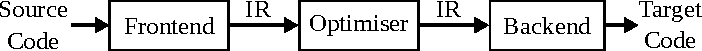
\includegraphics[scale=0.9]{src/background/figs/3-phase-compiler.pdf}
  \caption{Overview of the three-phase compiler infrastructure.}
  \label{fig:3-phase-compiler}
\end{figure}

%The front end parses source code, checking it for errors, and builds a language-specific Abstract Syntax Tree (AST) to represent the input code. The AST is optionally converted to a new representation for optimization, and the optimizer and back end are run on the code.
%The optimizer is responsible for doing a broad variety of transformations to try to improve the code's running time, such as eliminating redundant computations, and is usually more or less independent of language and target.


\begin{figure}[h]
  \centering
  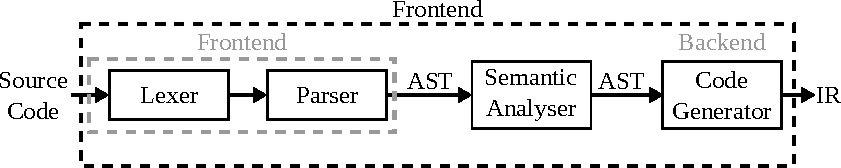
\includegraphics[scale=0.9]{src/background/figs/compiler-frontend.pdf}
  \caption{Overview of the three-phase compiler infrastructure.}
  \label{fig:compiler-frontend}
\end{figure}

\begin{figure}[h]
  \centering
  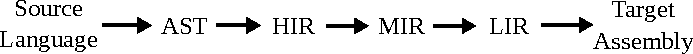
\includegraphics[scale=0.9]{src/background/figs/ir-lowering-sequence.pdf}
  \caption{Overview of the three-phase compiler infrastructure.}
  \label{fig:ir-lowering-sequence}
\end{figure}

\subsection{Link-Time Optimisations}
%% benefits of LTO
%% challenges with LTO
%% mention partial LTO, such as ThinLTO

\begin{figure}[h]
  \centering
  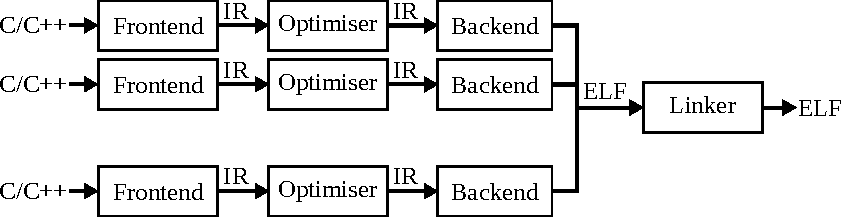
\includegraphics[scale=0.85]{src/background/figs/full-pipeline.pdf}
  \caption{Overview of the three-phase compiler infrastructure.}
  \label{fig:ir-lowering-sequence}
\end{figure}

\begin{figure}[h]
  \centering
  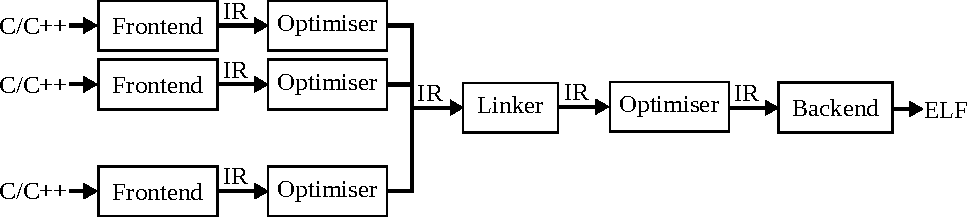
\includegraphics[scale=0.85]{src/background/figs/full-pipeline-LTO.pdf}
  \caption{Overview of the three-phase compiler infrastructure.}
  \label{fig:ir-lowering-sequence}
\end{figure}


\section{Optimisation Scope}
%% describe local optimisations (block level), global (intra-procedural), and inter-procedural (across functions)

\subsection{Interprocedural Optimisations}
%% benefits of IPO
%% challenges involved in IPO



\section{Sequence Alignment}

The comparison of two or more sequences, measuring the extent to which they differ, is important in many scientific areas, most notably in molecular biology~\cite{needleman70,smith81,carrillo88,wang94} where it has been critical
in the understanding of functional, structural, or evolutionary relationships between the sequences~\cite{kruskal83,mount05book}.

A particularly important comparison technique is sequence alignment, which identifies a series of patterns that appear in the same order in the sequences.
Essentially, sequence alignment algorithms insert blank characters in both input sequences so that the final sequences end up having the same size, where equivalent segments are aligned with their matching segments from the other sequence and non-equivalent segments are either paired with the blank or a mismatching character.

Figure~\ref{fig:seq-align-example} shows an example of a pair-wise sequence alignment.
This example, adapted from Lee~et~al.~\cite{lee02}, shows two protein sequences where amino acids are represented by their one-letter symbology~\cite{aasland68}.

\begin{figure}[h]
  \centering
  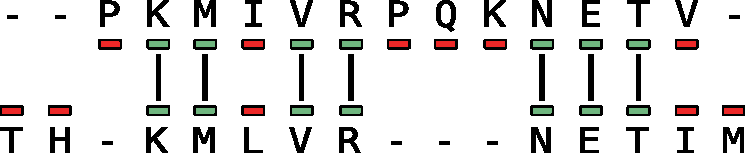
\includegraphics[scale=0.55]{src/background/figs/seq-align-example}
  \caption{Example of an optimum alignment between two sequences.
  Matching segments are shown in green, vertically centred, and the non-matching segments are shown in red at the sides.}
  \label{fig:seq-align-example}
\end{figure}

Formally, sequence alignment can be defined as follows:
For a given alphabet $\alpha$, a sequence $S$ of $k$ characters is an element of
$\alpha^k$, i.e., $S = (a_1, \ldots a_k)$.
Let $S_1, \ldots, S_m$ be a set of sequences, possibly of different lengths but
all derived from the same alphabet $\alpha$, where
$S_i = (a_1^{(i)}, \ldots, a_{k_i}^{(i)})$, for all $i\in\{1,\ldots,m\}$.
Consider an extended alphabet that includes the \textit{blank} character ``$-$'',
i.e., $\beta = \alpha \cup \{-\}$.
An alignment of the $m$ sequences, $S_1, \ldots, S_m$, is another set of sequences,
$\bar{S}_1, \ldots, \bar{S}_m$, such that each sequence $\bar{S}_i$ is obtained
from $S_i$ by inserting blanks in positions where some of the other sequences
have non-blank and possibly equivalent characters, for a given equivalence relation.
All sequences $\bar{S}_i$ in the alignment set have the same length $l$, where
$\max\{k_1,\ldots,k_m\} \leq l \leq k_1 + \cdots + k_m$.
Moreover, $\forall i\in\{1,\ldots, m\}$, $\bar{S}_i = (b_1^{(i)},\ldots,b_l^{(i)})$,
there are increasing functions $v_i: \{1,\ldots,k_i\} \to \{1,\ldots,l\}$, such that:
\begin{itemize}
\item $b_{v_i(j)}^{(i)} = a_j^{(i)}$, for every $j \in \{1,\ldots,k_i\}$;
\item any position not covered by the function $v_i$ contain a black character, i.e., for every $j \in \{1,\ldots,l\}\setminus \textrm{Im} \, v_i$, $b_j$ is the blank character ``$-$''.
\end{itemize}
Finally, for all $j\in\{1,\ldots,l\}$, there is at least one value of $i$ for which $b_j^{(i)}$ is not a blank character.
Note that two aligned sequences may contain both non-blank and non-equivalent characters at any given position, in which case there is a mismatch.

The sequence alignment problem is concerned with identifying an alignment that maximises the score for a given scoring scheme.
The scoring scheme first defines a weight for the alignment of pairs of characters which will then be used to compose a score for the whole sequence alignment.
These weights are used to penalise mismatches and gaps while favouring matching pairs.

The alignment score between two characters is defined by a function on pairs of characters, $\delta \in \beta\times\beta \to \mathbb{R}$, for a given extended alphabet $\beta$.
The simplest function that is commonly used is the constant function~\cite{haque09}.
Let $a,b\in\beta$ and $a \neq b$.
This constant function is defined by a triple $(w_1,w_2,w_3)\in\mathbb{R}^+\times\mathbb{R}^-\times\mathbb{R}^-$, such that:
\begin{itemize}
\item For two matching caracters, $\delta(a,a) = w_1, w_1\in\mathbb{R}^+$.
\item For a mismatch betweem non-blank characters, $\delta(a,b) = w_2, w_2\in\mathbb{R}^-$.
\item The gap penalty, for when we have a blank character, $\delta(a,-) = \delta(-,a) = w_3, w_3\in\mathbb{R}^-$.
\end{itemize}
This is a simple scoring scheme that rewards matches and penalises mismatches and gaps.

There is a vast literature on algorithms for performing sequence alignment, especially in the context of molecular biology.
These algorithms are classified as either global or local.
A global sequence alignment algorithm attempts to align the entire sequence, using as many characters as possible, up to both ends of each sequence.
Global alignment algorithms are useful for sequences that are highly similar and have approximately the same length~\cite{mount05book}.
Alternatively, a local sequence alignment algorithm generates subalignments in stretches of sequence with the highest density of matches.
Local alignments are more suitable for aligning sequences with very few similarities or vastly different lengths~\cite{mount05book}.

In this work, we will focus on pair-wise global alignment algorithms.
The following sections describe the main optimal algorithms based on dynamic programming.
These algorithms will offer different optimality, performance, and memory usage trade-offs~\cite{needleman70,smith81,carrillo88,hickey11}.
%Different alignments would produce different but valid merged functions.

\subsection{Needleman-Wunsch Algorithm}

The Needleman-Wunsch algorithm~\cite{needleman70} is one of the most well known algorithm for pair-wise global alignment.
This algorithm gives an alignment that is guaranteed to be optimal for a given scoring scheme~\cite{higgins89}.

The Needleman-Wunsch algorithm is based on dynamic programming and consists of two main steps.
First, it builds a \textit{similarity matrix}, based on a scoring scheme, which assigns weights for matches, mismatches, and \textit{gaps} (blank characters).
Afterwards, a backward traversal is performed on the similarity matrix, in order to reconstruct the final alignment by maximizing the total score.

\begin{figure}[h]
  \centering
  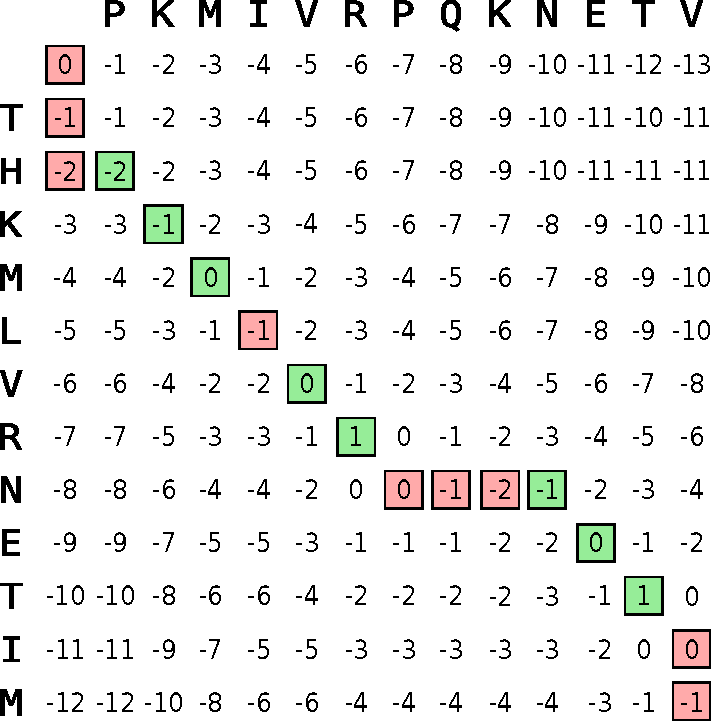
\includegraphics[scale=0.6]{src/background/figs/seq-align-example-nw}
  \caption{Example of the \textit{similarity matrix} computed for two input sequences.
           The highlighted cells represent the resulting alignment computed by the Needleman-Wunsch algorithm.}
  \label{fig:seq-align-example-nw}
\end{figure}

Figure~\ref{fig:seq-align-example-nw} shows the similarity matrix corresponding to the example from Figure~\ref{fig:seq-align-example}.
The similarity matrix is constructed by comparing all possible pairs of characters from the input sequences.
Let $S_1$ and $S_2$ be our input sequences of sizes $k_1$ and $k_2$, respectively, where $S_1 = (a_1,\ldots,a_{k_1})$ and $S_2 = (b_1,\ldots,b_{k_2})$.
The similarity matrix $M$ computed for these two input sequences will have size $(k_1 + 1) \times (k_2+1)$.
Let $M_{i,j}$ denote all entries in the similarity matrix, with $1 \leq i \leq (k_1 + 1)$ and $1 \leq j \leq (k_2 + 1)$.
The first entry in the matrix is $M_{1,1} = 0$, and
\begin{equation*}
%\begin{align*}
M_{i,j} = \max \begin{cases}
  M_{i-1,j} + \delta(a_{i-1},-)         &  \quad  \text{if } i>1 \text{ and } j\geq1 \\
  M_{i,j-1} + \delta(-,b_{j-1})         &  \quad  \text{if } i\geq1 \text{ and } j>1 \\
  M_{i-1,j-1} + \delta(a_{i-1},b_{j-1}) &  \quad  \text{if } i>1 \text{ and } j>1
\end{cases}
%\end{align*}
\end{equation*}
In other words, the score for each cell in the similarity matrix is the maximum among the rules shown in Figure~\ref{fig:seq-align-rules}.

\begin{figure}[h]
  \centering
  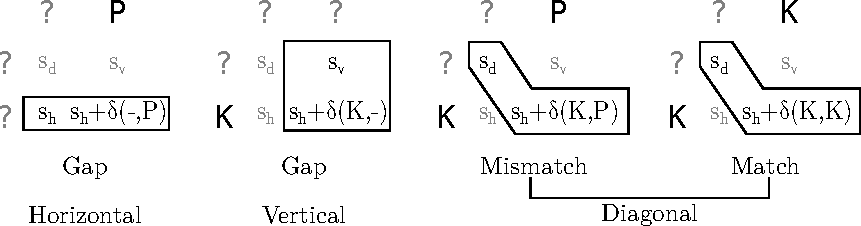
\includegraphics[scale=0.8]{src/background/figs/seq-align-rules}
  \caption{Set of rules used to compute the scores of the similarity matrix.
           The two first rules represent the penalty of inserting a horizontal or vertical gap.
           The diagonal rule depends whether we have a matching or mismatching pair of input characters.}
  \label{fig:seq-align-rules}
\end{figure}


Figure~\ref{fig:seq-align-example-nw} also highlights the traversal. 
Note that sometimes, while traversing the score matrix, there are multiple adjacent neighbours with the same score.
Since there may exist multiple traversals with the same score, two sequences can have multiple optimum alignments.

Needleman-Wunsh algorithm is quadratic in the size of the sequences being aligned, both in time and space.

%\subsection{Hirschberg Algorithm}

\chapter{Related Work}

\section{Code-Size Optimisations}

Although initially motivated by performance, many of the classical optimisations achieve better performance by reducing code size.
A small code, besides having fewer instructions to execute, can also have a positive impact on the cache utilisation.
Classical optimisations that are effective in reducing code size include the elimination of redundant, unreachable, and dead code, as well as certain kinds of strength reduction~\cite{cocke70,briggs97,debray00}.
In this section, we will describe some of these classical size-reducing optimisations.

\subsection{Constant Folding}

Constant folding is an optimisation that operates on the instruction level, identifying instructions whose operands are constant values, performing the evaluation of the instruction at compile time, and replacing it by the resulting value.
The effectiveness of constant folding can be augmented by combining it with constant propagation.
Constant folding reduces code size by eliminating instructions that can be computed at compile time.
Moreover, constant folding also works as an enabler to other optimisations, such as unreachable-code elimination (Section~\ref{sec:relatedwork:unreachable}).
 
\subsection{Unreachable-Code Elimination} \label{sec:relatedwork:unreachable}

Some functions may contain code that is unreachable. A code is unreachable if there is no valid control-flow path from the function's entry point that leads to it.
Since unreachable code is guaranteed to never be executed, compilers should remove it to avoid code bloat.

Often, unreachable code is uncovered by other optimisations.
For example, after constant propagation and constant folding, a conditional branch could have its condition evaluating to a constant, eliminating a path to one of its successor basic block.
If no other path leads to that basic block, it becomes unreachable.

The algorithm to eliminate unreachable code works in a mark-sweep manner, performing two passes over the basic blocks of the CFG.
The reachability analysis optimistically assumes that all basic blocks are dead until proven otherwise.
First, it marks all blocks as unreachable.
Next, starting from the entry point, it marks each block that it can reach as reachable.
If all branches and jumps are unambiguous, then all unmarked blocks can be deleted.
With ambiguous branches or jumps, the compiler must preserve any block that the branch or jump can reach.
This analysis is simple and inexpensive.

\subsection{Dead-Code Elimination}

A value definition is dead if it is not used on any path from the point in which it is defined to the exit point of the function.
In a similar way, an instruction is dead if it computes only values that are not used on any execution path leading from the instruction.
Any dead definition or instruction can be simply removed without altering the program's semantics, therefore reducing code size~\cite{muchnick98}.

The algorithm to eliminate dead code has some similarities with that for unreachable-code elimination described in Section~\ref{sec:relatedwork:unreachable}.
This algorithm also works in a mark-sweep manner~\cite{cooper07}.
First, the algorithm marks \textit{critical} instructions as \textit{alive}.
An instruction is \textit{critical} if it has an observable effect, for example, if it is a return instruction, a branch instruction, a function call, a memory operation, any instruction with side effect, etc.
Then, the algorithm follows the \textit{use-def chain} of every alive instruction, marking the operand instructions as alive.
This process continues until no more instructions can be marked as alive.
Finally, the sweep phase removes all instructions that have not been marked as alive, reducing code size.

\section{Merging Identical Functions}

In this section, we will discuss existing optimisations for merging identical functions.
Figure~\ref{fig:example-identical} illustrates how identical functions can appear in real programs.
The first pair of functions, shown in Figure~\ref{fig:example-identical-1-sphinx3}, were extracted from the \texttt{482.sphinx3} benchmark.
The only difference between these two functions is in their parameter type.
However, all pointer types can be considered equivalent since they can be bitcasted in a losslessly way.
These functions are usually produced by copy-and-paste programming, where a given code pattern is copied and then repurposed~\cite{kim04,jablonski10,ahmed15}.
The second pair of functions, shown in Figure~\ref{fig:example-identical-2-gcc}, were extracted from the \texttt{403.gcc} benchmark and they are fully identical.
These functions are part of GCC's backend, where it is common to have code that is automatically generated from a machine description~\cite{muchnick98,kolek13,ghica15}.

\begin{figure}[h]
\centering
\begin{subfigure}{\textwidth}
\centering
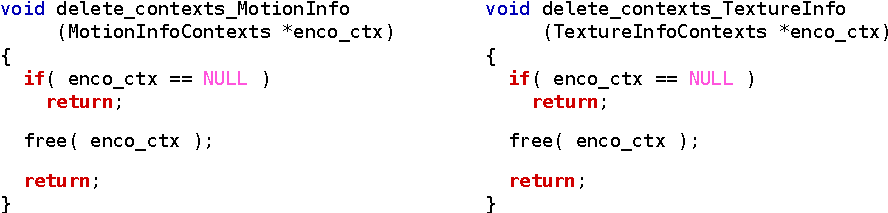
\includegraphics[scale=0.9]{src/relatedwork/figs/example-identical-1-sphinx3}
\caption{Two semantically identical functions extracted from the \texttt{482.sphinx3} benchmark.}
\label{fig:example-identical-1-sphinx3}
\end{subfigure}
\begin{subfigure}{\textwidth}
\centering
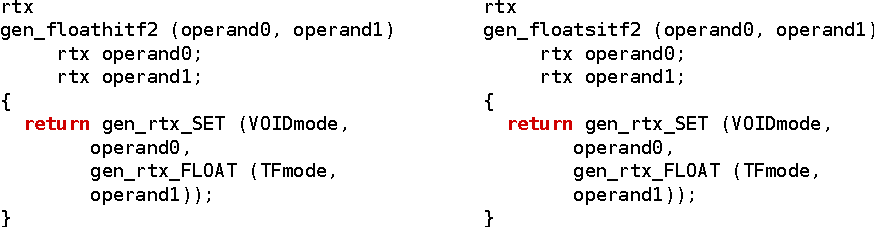
\includegraphics[scale=0.9]{src/relatedwork/figs/example-identical-2-gcc}
\caption{Two semantically identical functions extracted from the \texttt{403.gcc} benchmark.}
\label{fig:example-identical-2-gcc}
\end{subfigure}
\caption{Example of identical functions.}
\label{fig:example-identical}
\end{figure}

\begin{figure}[h]
\centering
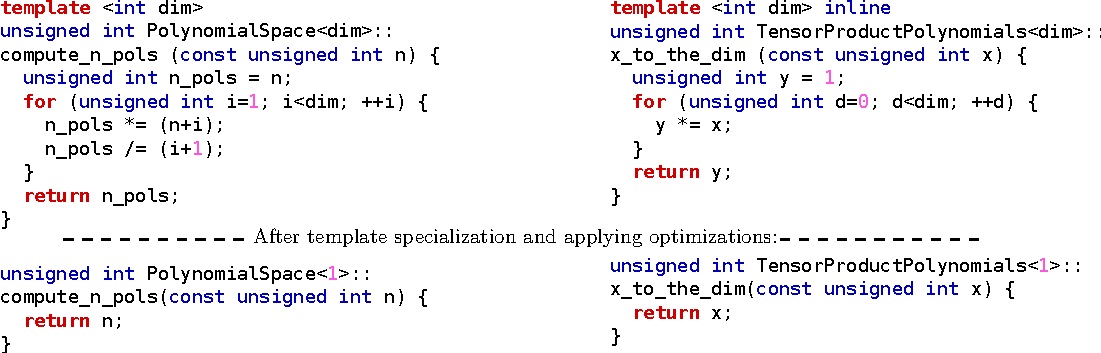
\includegraphics[scale=0.9]{src/relatedwork/figs/identical-example}
\caption{Two function extracted from the \texttt{447.dealII} benchmark that are not identical at the source level, but after applying template specialisation and optimisations they become identical at the IR level.}
\label{fig:identical-example}
\end{figure}

Note, however, that functions can be identical at the IR or machine level without necessarily being identical at the source level.
Figure~\ref{fig:identical-example} shows two real functions extract from the
447.dealII program in the SPEC CPU2006~\cite{spec} benchmark suite.
Although these two functions are not identical at the source level, they become
identical after a template specialisation and some optimisations are applied, in
particular, constant propagation, constant folding, and dead-code elimination. 
Specialising \verb|dim| to $1$ enables to completely remove the loop in the
function \verb|PolynomialSpace|.
Similarly, specializing \verb|dim| to $1$ results in only the first iteration
of the loop in the function \verb|TensorProductPolynomials| being executed.
The compiler is able to statically analyze and simplify the loops in both
functions, resulting in the identical functions shown at the bottom of
Figure~\ref{fig:identical-example}.

Identical code is particularly common in C++ programs
with heavy use of \textit{parametric polymorphism}, via template or \textit{auto} type deduction.



\section{Merging Identical Object Code}

The simplest way of merging identical functions is by looking at their object code, during link time.
\textit{Identical code folding}~(ICF) is an optimisation that identifies and merges two or more read-only sections, typically functions, that have identical contents.
This optimisation is commonly found in major linkers, such as \textit{gold}~\cite{tallam10,kwan12}, LLVM's \textit{lld}, and the MSVC linker~\cite{msvc-icf}.

Figure~\ref{fig:icf-example} shows an example, adapted from Tallam~\etal~\cite{tallam10},
of how generic programming in C++ can lead to identical functions in the object file.
The C++ code in in Figure~\ref{fig:icf-example-code} presents
a simple \textit{template class} and its member function being
instantiated multiple times with different pointer types.
Figure~\ref{fig:icf-example-object} shows the object code 
targeting the Intel x86 architecture.
For each instantiation of \textit{Foo}, a replica of its member
function \textit{getElement} is created.
Because the size of the different pointer types is the same,
all replicas of \textit{getElement} are identical
in the object file, which can be easily confirmed by
comparing their binary representation. as shown in
Figure~\ref{fig:icf-example-object}.

\begin{figure}[h]
% \begin{tabular}{cc}
% \begin{subfigure}{.5\textwidth}
% \begin{minted}[
% frame=lines,
% framesep=2mm,
% baselinestretch=1,
% %bgcolor=LightGray,
% fontsize=\footnotesize,
% %linenos
% ]{c++}
% template<typename T>
% class Foo {
%   ...
%   T element;
% public:
%   ...
%   T getElement() {
%     return element;
%   }
% };

% int main() {
%   Foo<int *> p;
%   Foo<float *> q;
%   Foo<void *> r;
%   ...
%   auto *pptr = p.getElement();
%   auto *qptr = q.getElement();
%   auto *rptr = r.getElement();
%   ...
% }
% \end{minted}
% \caption{A \textit{template class} with several instantiations.}
% \label{fig:icf-example-code}
% \end{subfigure} &
% \begin{subfigure}{.5\textwidth}
% \vspace{10ex}
% \begin{minted}[
% escapeinside=||,
% %fontfamily=tt,
% frame=lines,
% framesep=2mm,
% baselinestretch=1,
% %bgcolor=LightGray,
% fontsize=\scriptsize,
% %linenos
% ]{nasm}
% ; Disassembly of Foo<int *>::getElement()
% section .text._ZN3FooIPiE10getElementEv:
% _ZN3FooIPiE10getElementEv:   ; Hex Code
%   mov  rax,QWORD PTR [rdi]  ; 48 8b 07
%   ret                        ; c3

% ; Disassembly of Foo<float *>::getElement()
% section .text._ZN3FooIPfE10getElementEv:
% _ZN3FooIPfE10getElementEv:   ; Hex Code
%   mov  rax,QWORD PTR [rdi]  ; 48 8b 07
%   ret                        ; c3

% ; Disassembly of Foo<void *>::getElement()
% section .text._ZN3FooIPvE10getElementEv:
% _ZN3FooIPvE10getElementEv:   ; Hex Code
%   mov  rax,QWORD PTR [rdi]  ; 48 8b 07
%   ret                        ; c3
% \end{minted}
% \vspace{7ex}
% \caption{Disassembled object file.}
% \label{fig:icf-example-object}
% \end{subfigure}
% \end{tabular}
\caption{Example showing how a member function of a \textit{template class}
  can produce code replication susceptible to \textit{identical code folding}.
  For each instantiation of \textit{Foo}, a replica of the function
  \textit{getElement} is created for the template instance.
  When instantiated with pointer types, the object code of these functions will be identical.}
\label{fig:icf-example}
\end{figure}

Most object file formats, such as the \textit{Executable and Linkable Format} (ELF)~\cite{tallam10,kwan12}, are structured as separate sections of content, each section containing a certain type of content.
The main types are code segment, different types of data segment, and relocation information.
Relocation information describes how to modify other sections, connecting symbolic references to their definition.
In other words, it assigns actual addresses for position-dependent code and data.
For example, when a program calls a function, the associated call instruction must transfer control to the proper destination address at execution.

It is common practice for linkers to place functions in separate sections, as exemplified in Figure~\ref{fig:icf-example-object}.
Therefore, merging identical functions can be generalised to the problem of merging identical sections.
Two sections are considered identical if they have the identical section flags, data, code, and relocations.
Two relocations are considered the identical if they have the same relocation types, values, and if they point to the same or identical sections.

Since this equality has a cyclic definition, ICF is defined as a fixed-point computation, i.e., it is applied repeatedly until a convergence is obtained.
There are two approaches with distinct trade-offs.
$(i)$ The pessimistic apprach starts with all sections marked as being different and then repeatedly compare them trying to prove their equality, grouping those found to be identical, including their relocations.
This approach is implemented in the widely used \textit{gold} linker.
$(ii)$ The optimistic apprach starts with all functions marked as potentially identical and then repeatedly compare trying to disprove their equality, partitioning those found to be different.
This approach is implemented in LLVM's linker, \textit{lld}.

% \subsection{The Pessimistic Algorithm}

% The pessimistic algorithm is implemented in the gold linker.

% We can start with marking all functions as different and repeatedly do
% the checksumming.  This has the advantage that we do not need to wait
% for convergence. We can stop at any point and correctness will be
% guaranteed although not all cases would have been found.  However, this
% has a problem that some cases can never be found even if it is run until
% convergence.  Here is an example with mutually recursive functions :

% int funcA (int a)            int funcB (int a)
% {                            {
%   if (a == 1)                  if (a == 1)
%     return 1;                    return 1;
%    return 1 + funcB(a - 1);     return 1 + funcA(a - 1);
% }                            }

% In this example funcA and funcB are identical and one of them could be
% folded into the other.  However, if we start with assuming that funcA
% and funcB are not identical, the algorithm, even after it is run to
% convergence, cannot detect that they are identical.


% \subsection{The Optimistic Algorithm}

% The optimistic algorithm is implemented in LLVM linker, lld.

\begin{figure}[h]
% \begin{tabular}{cc}
% \begin{subfigure}{.5\textwidth}
% \begin{minted}[
% frame=lines,
% framesep=2mm,
% baselinestretch=1,
% %bgcolor=LightGray,
% fontsize=\footnotesize,
% %linenos
% ]{c++}
% int zip() {
%   return 0;
% }
% int zap() {
%   return 0;
% }
% int foo() {
%   return zip ();
% }
% int bar() {
%   return zap ();
% }
% \end{minted}
% \caption{A \textit{template class} with several instantiations.}
% \label{fig:icf-example-code}
% \end{subfigure} &
% \begin{subfigure}{.5\textwidth}
% \begin{minted}[
% escapeinside=||,
% frame=lines,
% framesep=2mm,
% baselinestretch=1,
% %bgcolor=LightGray,
% fontsize=\scriptsize,
% %linenos
% ]{gas}

% section .text._Z3zipv:
% _Z3zipv:                 ; Hex Code
%  xor eax, eax            ; 31 c0
%  ret                     ; c3    

% section .text._Z3zapv:
% _Z3zapv:
%  xor eax, eax            ; 31 c0
%  ret                     ; c3

% section .text._Z3foov:
% _Z3foov:
%  push rax                ; 50
%  call   6 |<\_Z3foov+0x6>|  ; e8 00 00 00 00
%  pop rcx                 ; 59
%  ret                     ; c3
% section .rela.text._Z3foov ; Relocation
% ; Type         Addend  Name
%  X86_64_PC32    -4      _Z3zipv

% section .text._Z3barv:
% _Z3barv:
%  push rax                ; 50
%  call   6 |<\_Z3barv+0x6>|  ; e8 00 00 00 00
%  pop rcx                 ; 59
%  ret                     ; c3
% section .rela.text._Z3barv ; Relocation
% ; Type         Addend  Name
%  X86_64_PC32    -4      _Z3zapv

% \end{minted}
% \caption{Disassembled object file.}
% \label{fig:icf-example-object}
% \end{subfigure}
% \end{tabular}
\begin{subfigure}{\textwidth}
\centering
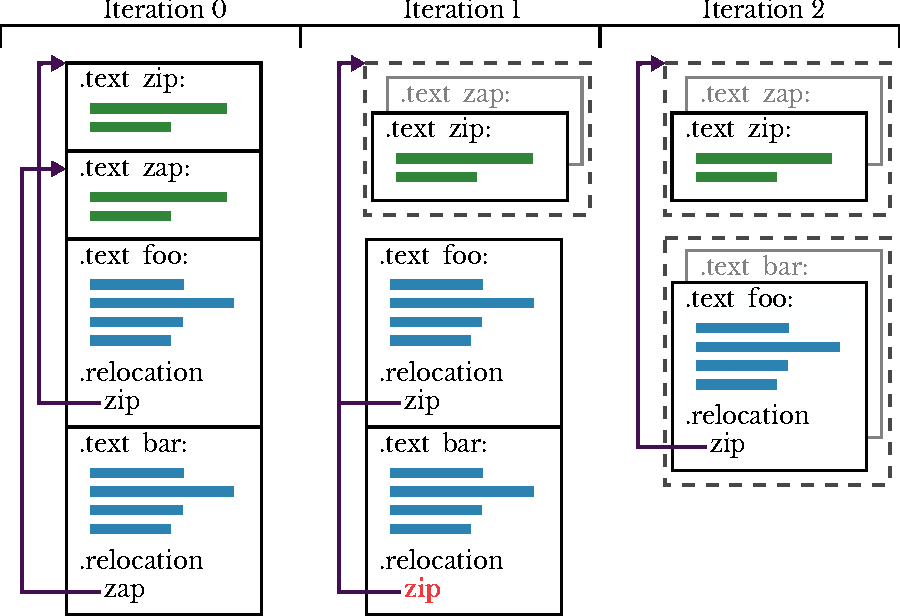
\includegraphics[width=0.9\textwidth]{src/relatedwork/figs/icf-example}
\caption{.}
\label{fig:identical-example}
\end{subfigure}

\caption{Example showing how a member function of a \textit{template class}
  can produce code replication susceptible to \textit{identical code folding}.
  For each instantiation of \textit{Foo}, a replica of the function
  \textit{getElement} is created for the template instance.
  When instantiated with pointer types, the object code of these functions will be identical.}
\label{fig:icf-example}
\end{figure}


\subsection{Identical Function Merging}

A similar optimisation for merging identical functions, but instead at the
intermediate representation (IR) level, is also offered by both GCC and
LLVM~\cite{llvm-fm,livska14}.
%The function merging optimisation currently offered by LLVM is only able to
%merge identical functions.
This optimisation is only flexible enough to accommodate simple type mismatches
provided they can be bitcasted in a losslessly way.

%%%%%%%%%%%%%%%%%%%%%%%%%%%%%%%%%%%%%%%%%%%%%%%%%%%%%%%%%%%%%%%%%%%%%%%%%%%%%%%%

A very strict function comparator is used to identify if two functions are 
semantically equivalent.
First it compares the signature and other general attributes of the two functions.
The functions must have identical signature, i.e., the same return type, the same
number of arguments, and exactly the same list of argument types.
Then this function comparator performs a simultaneous walk, in depth
first order, in the functions' control-flow graphs.
This walk starts at the entry block for both functions, then takes each block
from each terminator in order.
As an artifact, this also means that unreachable blocks are ignored.
Finally, it iterates through each instruction in each basic block.
Two blocks are equivalent if they have equivalent instructions in exactly the
same order, without excess.
The comparator always fails conservatively, erring on the side of claiming that
two functions are different.

When a pair of equivalent functions is identified, we can create either
an alias or a \textit{thunk}.
Aliasing etails eliminating one of the functions and replacing all its callsites
to the other function.
Thunks must be created when neither of the equivalent functions can be eliminated
by aliasing.
In such case, a thunk is created for either one of the functions, replacing its
body by a call to the other function, which allows all callsites and name
references to both functions to be preserved.
%In such case, the body of one of the functions is replaced by a call to the
%other function, and all callsites to both functions are preserved.
Aliasing is prefered since it is cheaper and adds no runtime overhead.
The appropriate merging is applied according to following rules:
\begin{itemize}
\item If the address of at least one function is not taken, alias can be used.
\item But if the function is part of COMDAT section that can be replaced, we
must use thunk.
\item If we create a thunk and none of functions is writeable, we can redirect calls
instead.
\end{itemize}
%%%%%%%%%%%%%%%%%%%%%%%%%%%%%%%%%%%%%%%%%%%%%%%%%%%%%%%%%%%%%%%%%%%%%%%%%%%%%%%%
%Similarly to the technique proposed by Edler von Koch~et~al.~\cite{edler14},
%LLVM's optimisation also exploits structural similarity among functions.
%However, the current implementation does not allow instructions to differ in
%their opcodes or in the number and type of their input operands.
Although very restrictive, this optimisation guarantees that any pair of
mergeable functions will result in code size reduction with no performance
overhead.

%Its simplicity also benefits compilation time, as the actual merge operation
%is trivial.
Its simplicity also allows for an efficient exploration approach based on computing
a hash of the functions and then using a binary tree to identify equivalent
functions.
%%%%%%%%%%%%%%%%%%%%%%%%%%%%%%%%%%%%%%%%%%%%%%%%%%%%%%%%%%%%%%%%%%%%%%%%%%%%%%%%
%We define a congruent group as a set of functions that are candidates for
%function equality.
%To create congruent groups, we build a compound hash value for each previously
%parsed function.
%%%As an optimisation, a hash of the function structure is calculated first, and
%%%two functions are only compared if they have the same hash.
Since hashing is cheap to compute, it allows us to efficiently
%Hashing is used to
group possibly equivalent functions and filter out functions
that are obviously unique.
%This hash is cheap to compute,
This hash must have the property that if function $F = G$
according to the comparison function, then $hash(F) = hash(G)$.
Therefore, as an optimisation, two functions are only compared if they have the
same hash.
This consistency property is critical to ensuring all possible merging
opportunities are exploited.
Collisions in the hash affect the speed of the pass but not the correctness
or determinism of the resulting transformation.

A function hash is calculated by considering only the number of arguments and
whether a function is varargs, the order of basic blocks (given by the
successors of each basic block in depth first order), and the order of
opcodes of each instruction within each of these basic blocks.
This mirrors the strategy of compare() uses to compare functions by walking the BBs in depth
first order and comparing each instruction in sequence. Because this hash
does not look at the operands, it is insensitive to things such as the
target of calls and the constants used in the function, which makes it useful
when possibly merging functions which are the same modulo constants and call
targets.


All functions can be sorted based on their hash value, which ends up grouping
possibly equivalent functions together.
If the hash value of a given function matches any of its adjacent values in
the sorted list, this function must be considered for merging.
%After that, the pass sorts each function to a congruent class according to
%its hash value.
%All functions in the module, ordered by hash.
Functions with a unique hash value can be easily ignored since no other function
will be found equivalent.
%Functions with a unique hash value are also easily eliminated.
%Otherwise it is dropped and never considered again.


The functions that remain are inserted into a binary tree, where functions are
the node values themselves.
An order relation is defined over the set of functions.
We need total-ordering, so we need to maintain four properties on the functions set:
\begin{itemize}
\item $a <= a$ (reflexivity);
\item if $a <= b$ and $b <= a$ then $a = b$ (antisymmetry);
\item if $a <= b$ and $b <= c$ then $a <= c$ (transitivity);
\item for all $a$ and $b$, $a <= b$ or $b <= a$ (totality).
\end{itemize}
This total-ordering was made through special function comparison procedure that
returns:
\begin{itemize}
\item 0 when functions are semantically equal,
\item -1 when Left function is less than right function, and
\item 1 for opposite case.
\end{itemize}

Functions are kept on binary tree. For each new function F we perform
lookup in binary tree.

%After the previous step is finished, all candidates in a group must be proved to
%be really semantically equivalent.

%Therefore, by construction, functions are hashed and grouped in O(n log n) time
%complexity.






\section{Merging Beyond Identical Functions}

In the previous sections, we have seen compiler optimisations that merge identical functions.
However, nearly identical functions, with only minor differences, are also commonly found.
Figure~\ref{fig:example-similar} shows two examples of nearly identical functions found in real programs.
The highlighted differences prevent these functions from being merged by the identical function merging techniques.
%These functions are usually produced by copy-and-paste programming,
%where a given code pattern is copied and then repurposed~\cite{kim04,jablonski10,ahmed15}.
The first pair of functions, shown in Figure~\ref{fig:example-similar-1-hmmer}, illustrates code that is usually produced by copy-and-paste programming,
where a given code pattern is copied and then repurposed~\cite{kim04,jablonski10,ahmed15}.
The second pair of functions, shown in Figure~\ref{fig:example-similar-3-gcc}, are produced by generative programming~\cite{czarnecki99,draheim04}, where their code was
automatically generated using a description language~\cite{ghica15}.

\begin{figure}[h]
\centering
\begin{subfigure}{\textwidth}
\centering
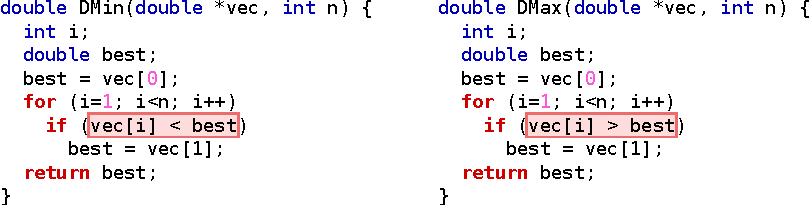
\includegraphics[width=0.9\textwidth]{src/relatedwork/figs/example-similar-1-hmmer}
\caption{Two similar functions extracted from the \texttt{456.hmmer} benchmark.}
\label{fig:example-similar-1-hmmer}
\end{subfigure}
%\begin{subfigure}{\textwidth}
%\centering
%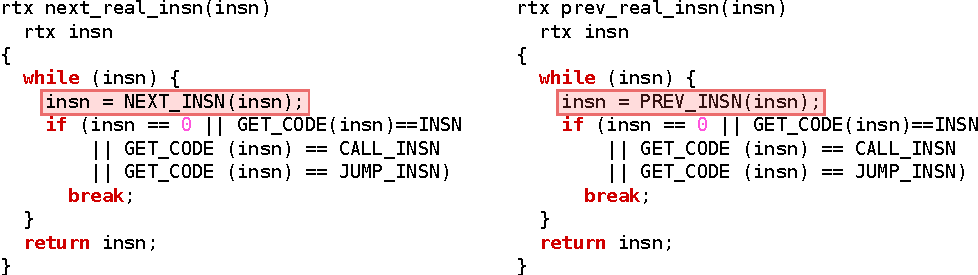
\includegraphics[width=0.9\textwidth]{src/relatedwork/figs/example-similar-2-gcc}
%\caption{Two similar functions extracted from the \texttt{403.gcc} benchmark.}
%\label{fig:example-similar-2-gcc}
%\end{subfigure}
\begin{subfigure}{\textwidth}
\centering
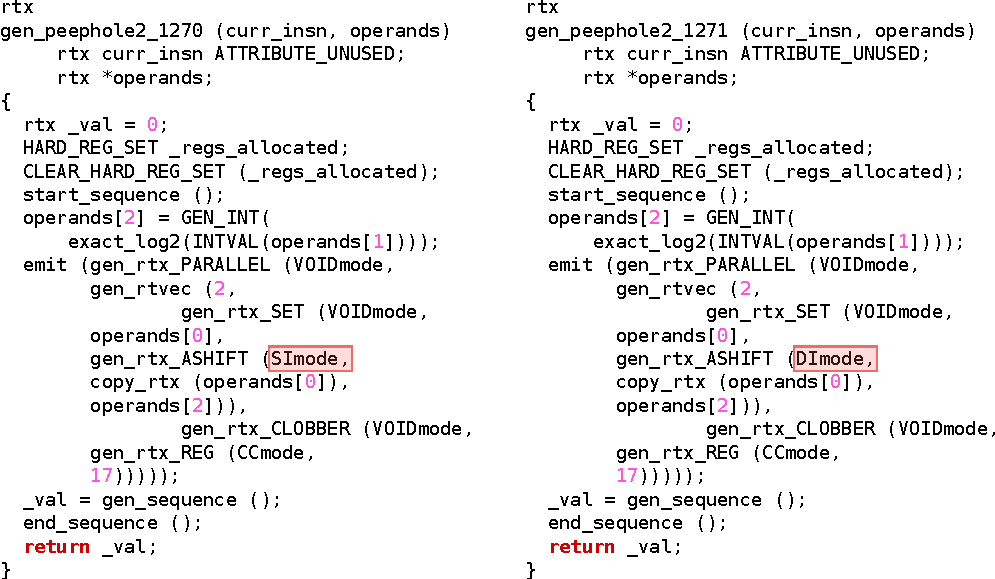
\includegraphics[width=\textwidth]{src/relatedwork/figs/example-similar-3-gcc}
\caption{Two similar functions extracted from the \texttt{403.gcc} benchmark.}
\label{fig:example-similar-3-gcc}
\end{subfigure}
\caption{Example of two pairs of highly similar functions. Because they are not identical, they cannot be merged by the function merging technique currently found in major compilers.}
\label{fig:example-similar}
\end{figure}


% The function merging technique presented in \cite{edler14} restricts merging to nearly identical functions.
% They only allow for pairs of corresponding instructions to differ if they still have equivalent data type.


Edler von Koch~et~al.~\cite{edler14} have proposed a function-merging technique which exploits structural similarity among functions.
Their optimization is able to merge nearly identical functions.
%similar functions that are not necessarily identical.
Two functions are structurally similar if both their function types are equivalent
and their CFGs are isomorphic.
Two function types are equivalent if they agree in the number, order, and types
of their parameters as well as
their return types, linkage type, and other compiler-specific properties.
In addition to the structural similarity of the functions, their technique also
requires that corresponding basic blocks have exactly the same number of instructions
and that corresponding instructions must have equivalent resulting types.
% but may differ in their opcodes or in the number and type of their input operands.
Mergeable functions are only allowed to differ in corresponding instructions,
where they can differ in their opcodes or in the number and type of their input operands.
Corresponding named values must have the same data type.
%The only differences that are actually allowed is that
%corresponding instructions can 
%differ in their opcodes or in the number and type of their input operands.


%If two corresponding instructions have different opcodes, they split the basic
%block and insert a switch branch to select which instruction to execute
%depending on a function identifier.

Because their technique is limited to functions with identical CFGs
and function types, once it merges a pair of functions, a third
\textit{similar} function cannot be merged into the resulting merged function
since they will differ in both CFGs and their lists of parameters.
Due to this limiting factor, the state-of-the-art has to first group
mergeable functions before simultaneously merging all functions within a group.

Their algorithm iterates simultaneously over corresponding basic
blocks in the set functions being merged, as they have isomorphic CFGs.
Figure~\ref{fig:soa-example-1} shows an example of two functions with isomorphic CFGs and their corresponding basic blocks arranged side by side.

\begin{figure}[h]
  \centering
  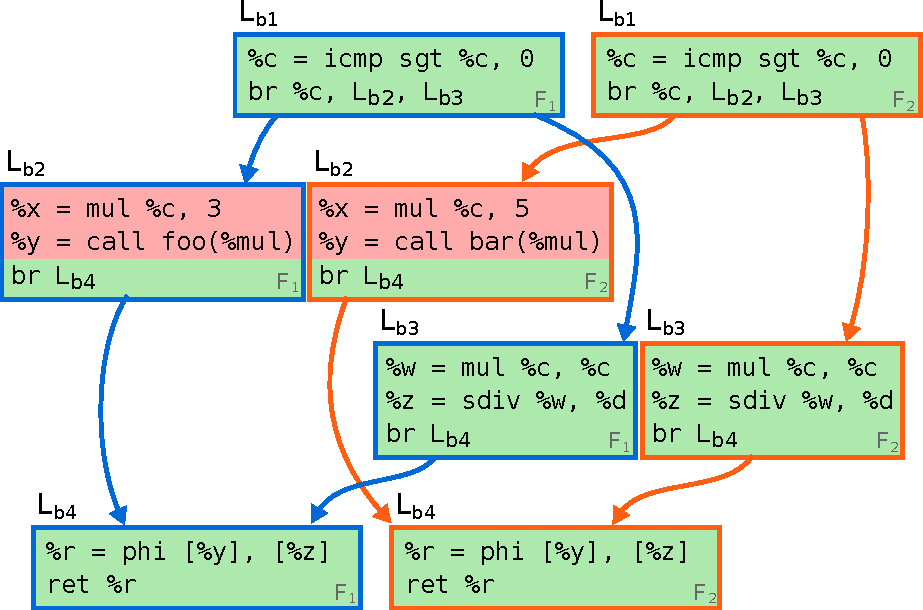
\includegraphics[width=0.8\textwidth]{src/relatedwork/figs/soa-example-1.pdf}
  \caption{An example of two functions with isomorphic CFGs and their corresponding basic blocks arranged side by side. Instructions in paired basic blocks are compared in a pairwise manner.}
  \label{fig:soa-example-1}
\end{figure}

Every pair of basic blocks have their instructions analysed in a pairwise manner.
Two instructions match if they have the same opcode with equivalent data types and operands.
Even if two instructions differ only on their operands, they are classified as mismatching.
For every pair of basic blocks, if their corresponding instructions have any difference, except for the data type of the computed value, the merged basic block is split by inserting a switch branch to select which instruction
to execute depending on a function identifier.
A phi-node is used to unify the mismatching instructions as a single named value.
This unification is only possible because they compute values of the equivalent data types.
Note that no operand selection is performed, every use of the mismatching instructions will refer to their phi-node.
Figure~\ref{fig:soa-example-2} shows an example of a merged basic block containing two mismatching pairs of instructions.
A split is added for every pair of mismatching instructions with the phi-node instruction added to the their immediate point of convergence.

% Because these instructions have equivalent resulting types, their results can be
% merged using a phi-operator, which can then be used transparently as operands
% by other instructions.

\begin{figure}[h]
  \centering
  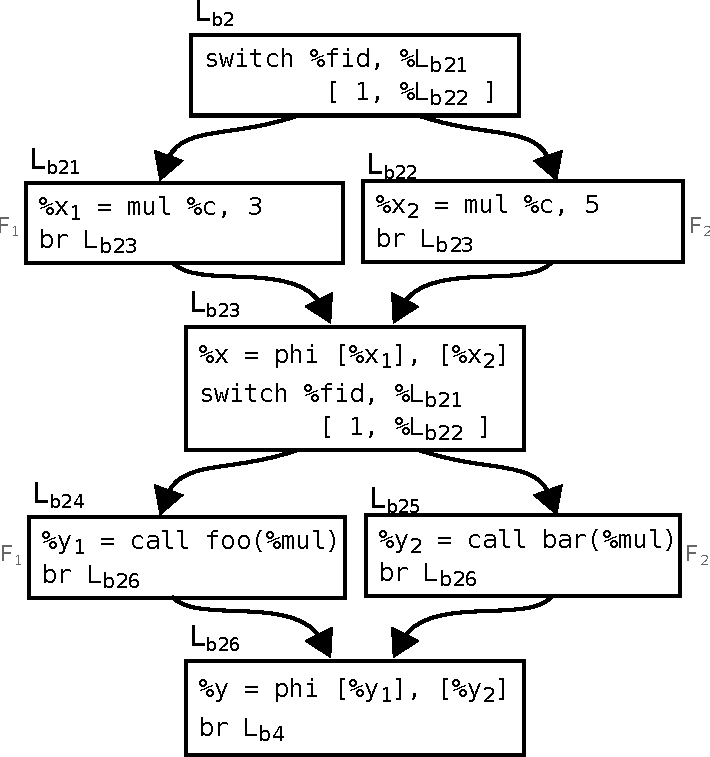
\includegraphics[width=0.6\textwidth]{src/relatedwork/figs/soa-example-2.pdf}
  \caption{An example of a merged basic block containing two mismatching pairs of instructions. A split is added for every pair of mismatching instructions with the phi-node instruction added to the their immediate point of convergence.}
  \label{fig:soa-example-2}
\end{figure}

Overall, except for mismatching pairs of instructions, the two functions must have identical function types, i.e., they must have the same return type and list of arguments, identical CFGs, with corresponding basic blocks having the same number of instructions.
Although this technique improves over LLVM's identical function merging, it is
still unnecessarily limited.
In Section~\ref{sec:motivation}, we showed examples of very similar real functions where the technique proposed by Edler von Koch~et~al.~\cite{edler14} fails to merge.
In Chapter~\ref{chp:cgo19} we introduce a novel technique that addresses such limitations improving on their technique across the board.

%%%%%%%%%%%%%%%%%%%%%%%%%%%%%%%%%%%%%%%%%%%%%%%%%%%%%%%%%%%%%%%%%%%%%%%%



\textbf{TODO: Comparison table: Identical vs VonKoch vs Ours}


\section{Code Factoring}

%Function merging and code factoring are different techniques for solving the
%same fundamental problem of duplicated code.
Code factoring refers to related techniques that address the same fundamental
problem of duplicated code in a different way.
%While the former works by merging similar functions, the latter works by
%factoring out duplicated code~\cite{loki04}.
%Instead of merging similar functions, code factoring works by factoring out
%duplicated code into separate functions~\cite{loki04}.
Code factoring can be applied at different levels of the program~\cite{loki04}.
Local factoring, also known as local code motion, moves identical instructions
from multiple basic blocks to either their common predecessor or successor,
whenever valid~\cite{knoop94,briggs94,loki04}.
Procedural abstraction %(or outlining)
finds identical code
that can be extracted into a separate function, replacing all replicated
occurrences with a function call~\cite{loki04,dreweke07}.

Procedural abstraction differs from function merging as it usually works on
single basic blocks or single-entry single-exit regions.
Moreover, it only works for identical segments of code, and every identical
segment of code is extracted into a separate new function.
Function merging, on the other hand, works on whole functions, which can be
identical or just partially similar, producing a single merged function.

However, all these techniques are orthogonal to the proposed optimization and
could complement each other at different stages of the compilation pipeline.




\section{Code Similarity}

Code similarity has also been used in other compiler optimizations or tools for
software development and maintenance.
In this section, we describe some of these applications.

Coutinho~et~al.~\cite{coutinho11} proposed an optimization that uses instruction
alignment to reduce divergent code for GPU.
They are able to fuse divergent branches that contain single basic blocks,
improving GPU utilization.
%reducing idle cores.

Similarly, analogous algorithms have also been suggested to identify the
differences between two programs, helping developers with source-code
management and maintenance~\cite{yang91,miller85}.
These techniques are applied in tools for source-code management, such as
the \textit{diff} command~\cite{miller85}.

Similar techniques have also been applied to code editors and IDEs~\cite{toomim04,sajnani16}.
For example,
SourcererCC~\cite{sajnani16} detects possible clones, at the source level, by
dividing the programs into a set of code blocks where each code block is itself
represented by a bag-of-tokens, i.e., a set of tokens and their frequencies.
Tokens are keywords, literals, and identifiers, but not operators.
Code blocks are considered clones if their degree of similarity is higher than
a given threshold.
In order to reduce the number of blocks compared, candidate blocks are filtered
based on a few of their tokens where at least one must match.

Our ranking mechanism uses an approach similar to SourcererCC, where we use
opcode frequencies and type frequencies to determine if two functions are
likely to have similar code.
However, we need a precise and effective analysis of code similarity when
performing the actual merge.
To this end, we use a sequence alignment technique.



\section{Tuning Compilers with Deep Learning}

There is been many work using machine learning as a heuristic for tuning runtime systems~\cite{andreasson02,wang09,castro11,rocha17,pereira17} and compilers~\cite{cavazos05,leather09,cummins17,wang18,mendis19}.

Cavazos and O'Boyle~\cite{cavazos05} propose the use of genetic algorithm to tune the heuristics of function inlining.
They use genetic algorithm to optimise the values for different features that control the inlining heuristic.
%Some of these features are the size of the callee and caller functions.
These features are chosen by the compiler writer and they define the maximum size allowed by the inlining transformation for the callee and the caller functions, the maximum size for callee functions that are hot or that should always be inlined, etc.
The optimised features are then used to define the rules of the inlining heuristic, describing which call sites should be allowed for inlining.
The fitness function of the genetic algorithm involves the actual runtime of the compiled program, rendering the feature optimisation process very costly.
However, their approach is able to achieve significant speedups over the baseline.

The quality of these features is critical to the improvements resulting from machine learning solutions.
Leather~et~al.~\cite{leather09} propose the use of genetic programming in order to also automate the selection of these features.
The feature space is described by a grammar and is then searched with genetic programming and predictive modelling, to avoid recompilation of the program for each step in searching the optimization space.
The genetic programming technique is used to generate features that are fed to a decision tree.
This machine learning solution form the decision-making heuristics for the loop-unrolling optimisation.
They show that the automated selection of features outperform hand-coded features, for the same machine learning procedure based on decision trees.

Cummins~et~al.~\cite{cummins17} propose DeepTune, which uses deep neural networks to learn optimization heuristics directly on raw code, unifying the search for features and decision-making heuristics into a single learning model.
Since the program, in its textual form, can be seen as a sequence of tokens of variable length, using a recurrent neural networks becomes a natural choice.
DeepTune has an LSTM-based language model that processes raw code, producing a fixed-size encoding which is then fed to a heuristic model based on a feed-forward neural network.

Mendis~et~al.~\cite{mendis19} propose Ithemal, a tool which uses deep neural networks to predict the throughput of a set of machine instructions.
Ithemal can be used as a cost model for compiler optimisations and code generation, aiding the decision of whether a transformation would result in faster code.
Similar to DeepTune, Ithemal also processes raw machine instructions using an LSTM-based language model.
However, Ithemal has an architecture with two LSTM stages.
The first LSTM processes the tokens that compose one instruction.
The second LSTM processes the encoded instructions that are produced by the first LSTM.
The output of the second LSTM is aggregated into the final throughput prediction.

\chapter{Merging Pairs of Functions}

%%%%%%%%%%%%%%%%%%%%%%%%%%%%%%%%% FMSA %%%%%%%%%%%%%%%%%%%%%%%%%%%%%%%%%%%%%%%%%

In this section, we describe the proposed function-merging technique.
Contrary to the state-of-the-art, our technique is able to merge any two
functions.
If the two functions are equivalent, i.e., identical, then the two functions
can be completely merged into a single identical function.
However, if the two functions differ at any point, an extra parameter is
required, so that the caller is able to distinguish between the functions. 
The two functions can differ in any possible way, including their list of
parameters or return types.
If the lists of parameters are different, we can merge them so that we are able
to uniquely represent all parameters from both functions.
If the return types are different, we can use an aggregate type to return values
of both types or return just the non-void type if the other one is void.
%However, in our current implementation, the only restriction is that both
%functions must have equivalent return types or one of them must be \textit{void}.

\begin{figure}[h]
  \centering
  %\vspace{-1ex}
  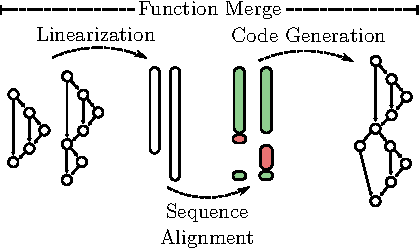
\includegraphics[width=0.85\linewidth]{src/merge-operation/figs/func-merge-overview.pdf}
  \caption{Overview of our function-merging technique.}
  \label{fig:func-merge-overview}
  %\vspace{-1ex}
\end{figure}

The proposed technique consists of three major steps, as depicted in
Figure~\ref{fig:func-merge-overview}.
First, we linearize each function, representing the CFG as a sequence of 
labels and instructions.
The second step consists in applying a sequence alignment algorithm, borrowed
from bioinformatics, which identifies regions of similarity between sequences.
The sequence alignment algorithm allows us to arrange two linearized functions
into segments that are equivalent between the two functions and segments where
they differ from one another.
The final step performs the code generation, actually merging the two functions
into a single function based on the aligned sequences.
Aligned segments with equivalent code are merged, avoiding redundancy, %redundant code,
and the remaining segments where the two functions differ have their code
guarded by a function identifier.
At this point, we also create a merged list of parameters where parameters of
the same type are shared between the functions, without necessarily keeping
their original order.
This new function can then be used to replace the original functions, as they
are semantically equivalent, given the appropriate function-identifier
parameter.

\subsection{Linearization}

The \textit{linearization}\footnote{Although linearization of CFGs
usually refers to a predicated representation, % resulting from an if-conversion,
in this paper, we refer to a simpler definition.}
of a function consits in specifying an ordering of the basic blocks based on a
traversal of the CFG and then producing a sequence of basic block labels and
instructions, similar to a textual representation of the function.
Although this operation is trivial, the specific ordering of the basic blocks
chosen can have an impact on the merging operation.

%For the linearization, we assume that every basic block has an entry label and
%a terminator instruction which refers explicitly to the successor basic blocks,
%if there are successors.
%This is true for most IRs, such as the LLVM IR, or can be easily adapted.

In our implementation, the linearization uses a reverse post-order~(RPO) of the
basic blocks, following a canonical ordering of the successors.
%, e.g., \textit{true} branches before \textit{false} ones.
%Figure~\ref{fig:branch-linearization} shows an example of the linearization 
%using the canonical RPO.
The RPO guarantees that the linearization starts with the entry basic block and
then proceeds favoring definitions before uses, except in the presence of loops.
Although the specifc ordering produced by the canonical linearization may not
be optimal, it is common practice for compilers to rely on prior
canonicalizations, e.g., 
canonical loops, canonical induction variables, canonical reassociation, etc.
For contrast, if, instead, we use an RPO linearization with a uniformly
randomized ordering of the successor basic blocks, the final code-size reduction
of the function-merging optimization can drop up to 10\% for individual
benchmarks.
Note that our decision for using the canonical RPO is purely pragmatic and
other orderings of the basic blocks could also be used, as long as it produces
a sequence of labels followed by instructions.

%\begin{figure}[h]
%  \centering
%  \includegraphics[width=0.6\linewidth]{figs/branch-linearization.pdf}
%  \caption{Linearization using a canonical reverse post-order.
%           The dashed arrows show where a randomized ordering could change the
%           linearization.}
%  \label{fig:branch-linearization}
%\end{figure}

\subsection{Sequence Alignment}

When merging two functions, the goal is to identify which pairs of instructions
and labels that can be merged and which ones need to be selected based on the
actual function being executed.
To avoid breaking the semantics of the original program, we also need to
maintain the same order of execution of the instructions for each one of
the functions.

To this end, after linearization, we reduce the problem of merging functions
to the problem of \textit{sequence alignment}. %~\cite{carrillo88,wang94}.
%After linearization, the problem of merging two functions can be reduced to the
%\textit{sequence alignment} problem~\cite{carrillo88,wang94}, which is itself
%closely related to finding the
%\textit{longest common subsequence}~\cite{hirschberg75,maier78}.
Sequence alignment is an important technique to many areas of science,
most notably in molecular biology~\cite{needleman70,smith81,carrillo88,wang94}
where, for example, it is used for identifying homologous subsequences of amino
acid in proteins.
Figure~\ref{fig:opcode-align} shows an example of the sequence alignment
between two linearized functions extracted from the \texttt{400.perlbench} benchmark
in SPEC CPU2006~\cite{spec}.

\begin{figure}[h]
  \centering
  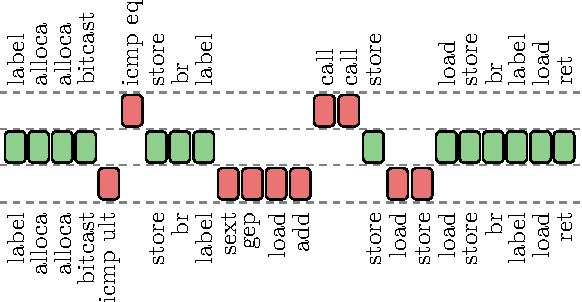
\includegraphics[width=0.85\linewidth]{src/merge-operation/figs/opcode-align.pdf}
  %\caption{An example of a sequence alignment between two real functions extracted from the \text{400.perlbench} benchmark.}
  \caption{The sequence alignment between two functions.}
  \label{fig:opcode-align}
\end{figure}

Formally, sequence alignment can be defined as follows:
For a given alphabet $\alpha$, a sequence $S$ of $k$ characters is a subset of
$\alpha^k$, i.e., $S = (a_1, \ldots a_k)$.
Let $S_1, \ldots, S_m$ be a set of sequences, possibly of different lengths but
all derived from the same alphabet $\alpha$, where
$S_i = (a_1^{(i)}, \ldots, a_{k_1}^{(i)})$, for all $i\in\{1,\ldots,m\}$.
%\begin{equation*}
%\begin{align*}
%S_1 = (a_1^{(1)}, \ldots, a_{k_1}^{(1)})\\
%\dots\\ 
%S_m = (a_1^{(m)}, \ldots, a_{k_m}^{(m)})
%\end{align*}
%\end{equation*}
Consider an extended alphabet that includes the \textit{blank} character ``$-$'',
i.e., $\beta = \alpha \cup \{-\}$.
An alignment of the $m$ sequences, $S_1, \ldots, S_m$, is another set of sequences,
$\bar{S}_1, \ldots, \bar{S}_m$, such that each sequence $\bar{S}_i$ is obtained
from $S_i$ by inserting blanks in positions where some of the other sequences
have non-blank and possibly equivalent characters, for a given equivalence relation.
All sequences $\bar{S}_i$ in the alignment set have the same length $l$, where
$\max\{k_1,\ldots,k_m\} \leq l \leq k_1 + \cdots + k_m$.
Moreover, $\forall i\in\{1,\ldots, m\}$, $\bar{S}_i = (b_1^{(i)},\ldots,b_l^{(i)})$,
there are increasing functions $v_i: \{1,\ldots,k_i\} \to \{1,\ldots,l\}$, such that:
\begin{itemize} %[noitemsep,topsep=0pt]
\item $b_{v_i(j)}^{(i)} = a_j^{(i)}$, for every $j \in \{1,\ldots,k_i\}$;
\item any position $j$ not mapped by the function $v_i$, i.e.,
for all $j \in \{1,\ldots,l\}\setminus \textrm{Im} v_i$,
then $b_j^{(i)}$ is a blank character.
\end{itemize}
Finally, for all $j\in\{1,\ldots,l\}$, there is at least one value of $i$ for
which $b_j^{(i)}$ is not a blank character.
%and for any pair of sequences that have a non-blank character at position $j$,
%these characters are equivalent.
Note that two aligned sequences may contain both non-blank and non-equivalent
characters at any given position, in which case it contains a mismatch.

Particularly for the function-merging, we are concerned with the alphabet
consisting of all possible typed instructions and labels.
Every linearized function represents a sequence derived from this alphabet.
We explain the equivalence relation used for this alphabet in the next section.

%We describe the equivalence relation between two predicated values in two
%separate cases, namely, the equivalence between instructions and the
%equivalence between labels.
%Labels are always considered equivalent.
%Two instructions are equivalent if their opcode are semantically equivalent,
%but not necessarily the same, and they both have types that can be bitcasted in
%a losslessly way from on to the other.
%This also includes making sure that there is no conflict regarding memory
%alignment when handling pointers.
%No additional restriction is imposed on the operands of the two instructions
%being compared for equivalence.
%Whenever two operands cannot be statically proved to represent the same value,
%a select instruction can be used to distinguish between the execution of two
%functions being merged.
%For function calls, the type equivalence requires that both instructions have
%identical function types, i.e., both called functions must have an identical
%return type and an identical list of parameter types. 

There is a vast literature on algorithms for performing sequence alignment,
especially in the context of molecular biology.
These algorithms range from optimal algorithms based on dynamic programming to
probabilistic models that does not guarantee
optimality~\cite{needleman70,smith81,carrillo88,hickey11}. 
In this paper, we use the Needleman-Wunsh algorithm~\cite{needleman70}.
This algorithm is based on dynamic programming and consists of two main steps.
First, it builds a \textit{similarity matrix}, based on a scoring scheme, which
assigns weights for matches, mismatches, and \textit{gaps} (blank characters).
Afterwards, a backward traversal is performed on the similarity matrix, in order
to reconstruct the final alignment by maximizing the total score.
We use a simple scoring scheme that rewards matches and penalizes mismatches and
gaps.

%\todo{Remove this paragraph.}
%When producing the final aligned sequence, there may be several possible optimal
%alignments.
%However, different aligned sequences can affect the code generation in different
%ways that may be both beneficial or undesirable. 
%For this reason, we prioritize alignments that tend to group the blank
%characters together, avoiding to frequently alternate between the two sequences
%during long segments of mismatches and gaps.
%For example, note that in Figure~\ref{fig:opcode-align}, the red blocks, for
%a particular sequence, tend to be grouped together.

\subsection{Equivalence Relation}

We describe the equivalence relation between values in two
separate cases, namely, the equivalence between instructions and the
equivalence between labels.

Labels can represent both normal basic blocks and landing blocks, which are used
in exception handling code.
Labels of normal basic blocks are always considered equivalent but
landing blocks must have exactly the same landingpad instructions.

Two instructions are equivalent if: $(1)$ their opcode are semantically
equivalent, but not necessarily the same; $(2)$ they both have equivalent types;
and $(3)$ they have pairwise operands with equivalent types.
Types are considered equivalent if they can be bitcasted in a losslessly way
from on to the other.
It is also important to make sure that there is no conflict regarding memory
alignment when handling pointers.
No additional restriction is imposed on the operands of the two instructions
being compared for equivalence.
Whenever two operands cannot be statically proved to represent the same value,
a select instruction is used to distinguish between the execution of two
functions being merged.
For function calls, the type equivalence requires that both instructions have
identical function types, i.e., both called functions must have an identical
return type and an identical list of parameter types. 

\subsubsection{Handling Exception Handling Code}

Most modern compilers implement the zero-cost Itanium ABI for exception
handling~\cite{dinechin00}, including GCC and LLVM, sometimes called the
\textit{landing-pad} model. In this section, we describe restrictions imposed
by exception handling code and their equivalence relation.

The invoke instruction co-operates tightly with its landing block, i.e., the
basic block pointed by the exception branch of an invoke instruction.
The landing block must landingpad instruction as its first non-$\phi$
instruction.
Given this restriction, two equivalent invoke instructions must also have
landing blocks with equivalent landingpad instructions.
This is easy to check since the landingpad instruction is always the first
instruction in a landing block. 

Landing blocks are responsible for handling all catch clauses of the
higher-level programming language covering the particular callsite.
All clauses are defined by the landingpad instruction, which encodes the list of
all exception and cleanup handlers.
Landingpad instructions are equivalent if they have the exactly same type and
also encode an identical lists of exception and cleanup handlers.
The type of equivalent landingpad instructions must be identical as its value
is crucial in deciding what action to take when the landing block is entered,
and corresponds to the return value of the personality function, which must also
be identical for the two functions being merged.

%The return value of the landingpad instruction is crucial in deciding what
%action to take when the landing block is entered, and corresponds to the return
%value of the personality function.

%In other words, when the unwinder executes the personality function (which
%is part of the language runtime), it stores its return value, and provides this return value in the result of the landingpad
%instruction. Since the personality function has access to the part of the unwind tables generated from the landingpad
%instruction, it can communicate information encoded in the unwind table to the landing block itself. In the libc++ runtime,
%the personality function returns a tuple consisting of a pointer to the exception object itself, and a “handler switch value”, an
%integer which corresponds to the index of a relevant “catch” clause of the landingpad instruction, or a special value (−1)
%when no catch clauses match but a cleanup needs to be performed.

%The LLVM IR generated for the landing block then checks the handler switch value computed by the personality function,
%and transfers control to a cleanup or handler block accordingly.

%Finally, if the selected handler is a cleanup handler, the
%exception propagation (stack unwinding) needs to be resumed after the cleanup is done. This is achieved by the resume
%instruction, which expects as a parameter the same value that was returned by the corresponding landingpad instruction
%which interrupted the exception propagation.
%Interestingly, there are no LLVM instructions for raising (throwing) exceptions. This is left entirely in the management
%of the language runtime, which needs to closely co-operate with the stack unwinding library anyway (the interface of the
%personality function is mandated by the stack unwinder).



%%%%%%%%%%%%%%%%%%%%%%%%%%%%%%%%%% SALSSA %%%%%%%%%%%%%%%%%%%%%%%%%%%%%%%%%%%%%%





Properly handling \textit{phi-nodes} requires a radical redesign in the code generator. The existing code generator produces code directly
from the aligned sequence, with each instruction pair treated almost in isolation without considering any control flow context. Merging
\textit{phi-nodes} cannot work with this approach because \textit{phi-nodes} are only understood in their control flow context.

\paragraph*{Road map} In the rest of this section, we describe {\ProjName}, our novel approach for merging functions through sequence alignment with full
support for the SSA form. By removing the need for preprocessing the input functions and performing register demoting, our approach is able
to merge functions better and faster. Instead of translating the aligned functions directly to merged code, the {\ProjName} follows a
top-down approach centered on the CFGs of the input functions. It iterates over the input CFGs, constructing the
CFG of the merged function, interweaving matching and non-matching instructions (Section~\ref{sec:code-gen-core}
). Afterwards, all edges and operands are resolved, including appropriately assigning the incoming values to all \textit{phi-nodes} (Section~\ref{sec:op-assign}).
{\ProjName} is designed to preserve all properties of SSA form via the standard SSA construction algorithm (Sections~\ref{sec:ssa-fix}).
Finally, {\ProjName} integrates a novel optimization with the SSA construction algorithm, called \textit{phi-node coalescing}, producing even smaller merged functions (Section~\ref{sec:pncoalescing}).

\begin{figure}[t!]
  \centering
  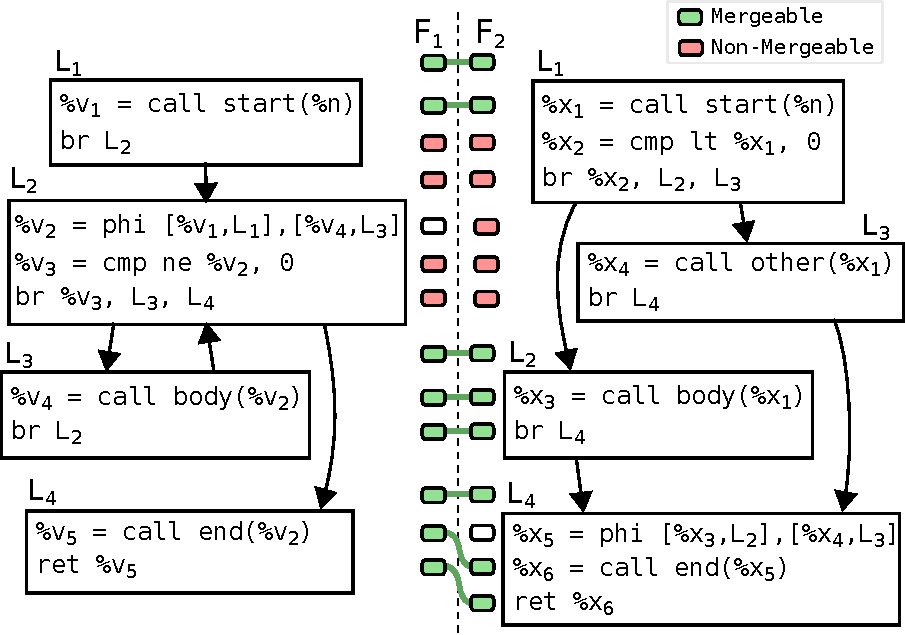
\includegraphics[scale=0.55]{src/merge-operation/figs/code-gen-cfg-input.pdf}
    \caption{Example of functions aligned without register demotion.
    \textit{Phi-nodes} are excluded from alignment.}
  \label{fig:code-gen-cfg-input}
\end{figure}

\paragraph*{Working examples} Figure~\ref{fig:code-gen-cfg-input} shows how the functions from our motivating example align without register demotion.
Here, \textit{phi-nodes} are not aligned, similarly to how FMSA handles \textit{landing-pad} instructions. We will use these as working
examples to describe step by step how our new code generator works in the next subsections.


\subsection{Control-Flow Graph Generation} \label{sec:code-gen-core}

\begin{figure}[t!]
  \centering
  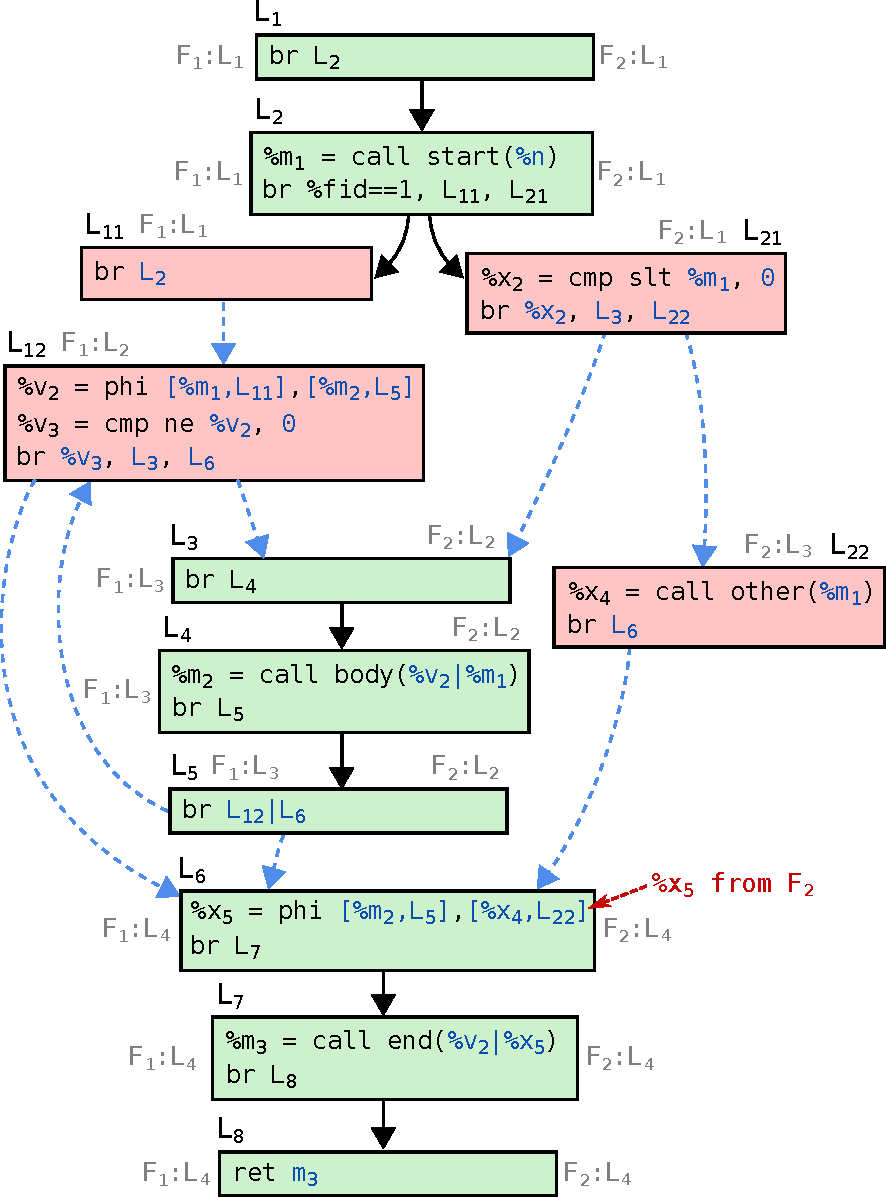
\includegraphics[scale=0.55]{src/merge-operation/figs/code-gen-cfg.pdf}
    \caption{Merged CFG produced by {\ProjName}. Code corresponding to a single
      input basic block may be transformed into a chain of blocks, separating
      matching and non-matching code. The generator inserts conditional and
      unconditional branches to maintain the same order of instructions
      from the input basic block. Operands and edges highlighted in blue will be
      resolved by the operand assignment described in Section~\ref{sec:op-assign}.}
  \label{fig:code-gen-cfg}
\end{figure}


Our code generator starts by producing all the basic blocks of the merged function.
Each original block is broken into smaller ones so that matching code is
separated from non-matching code and matching instructions and labels are placed
into their own basic blocks. Having one block per matching instruction or label
makes it easier to handle control flow and preserve the ordering of instructions
from the original functions by chaining these basic blocks as needed.

Blocks with instructions that come originally from the same basic block (of either input function) are chained in their original order with
branches. We use either unconditional branches or conditional branches on the function identifier depending on whether control flow out of
this code is different for the two input functions. Because we have one basic block per pair of matching instructions/labels, this tends to
generate some artificial branches, most of them are unconditional, but can be simplified in later stages.


%Our code generator starts by creating individual basic blocks for each pair of
%matching labels or instructions obtained from the resulting alignment.
%Afterwards, while generating the remaining and non-matching code from the input functions,
%these isolated basic blocks that represent matching code will also be chained
%together, following the order they originally appear in the input function.
%This chaining operation is performed separately for each function on a per
%basic block basis.

%For the first function, {\ProjName} iterates over each basic block, generating
%the remaining non-matching code.
%All matching and non-matching instructions generated from the same basic block
%are chained together via unconditional branches.
%As a result, each basic block from the input functions are represented by a
%sequence of basic blocks that contain either matching or non-matching
%instructions.

%Similarly, for each basic block in the second function, the non-matching
%code is generated and chained with the matching code that have already been
%generated.
%During this chaining process, if the control flow of a matching basic block
%differs from the one created for the first function,
%then {\ProjName} creates a conditional branch based on the function identifier,
%preserving the order of the instructions for both input functions.
%This process is trivial since we have the matching instructions in
%separate basic blocks and it suffices to change the branching instruction,
%selecting the correct control flow based on the function identifier.



Figure~\ref{fig:code-gen-cfg} shows the generated CFG. At this point, the only
instructions that actually have their operands assigned are the branches inserted
to chain instructions originating from the same input basic block.
These branches have no corresponding instruction in the input functions.
All other operands and edges, depicted in blue in Figure~\ref{fig:code-gen-cfg},
will be resolved later, during operand assignment.

\subsubsection{Phi-Node Generation}

Our code generator treats \textit{phi-nodes} differently from other instructions. For all alignment and code generation purposes,
{\ProjName} treats \textit{phi-nodes} as attached to their basic block's label; that is, they are aligned with their labels and are
copied to the merged function with their labels. So, when creating a basic block for a label, we also generate the \textit{phi-nodes}
associated with it. For a pair of matching labels, we copy all \textit{phi-nodes} associated with both labels.
We have decided for this approach where phi-nodes are tied to labels because phi-nodes describe primarily how data flows into its corresponding basic block.
%Figure~\ref{fig:code-gen-cfg} shows one such example, where both \textit{phi-nodes}, \texttt{v\textsubscript{2}} and
%\texttt{x\textsubscript{3}} are copied into \texttt{L\textsubscript{6}}, despite the fact it represents a pair of matching labels.
Figure~\ref{fig:code-gen-cfg} shows an example where \textit{phi-nodes} are present in basic blocks
with both matching or non-matching labels.
The phi-node \texttt{x\textsubscript{5}} is simply copied into the merged basic block labeled \texttt{L\textsubscript{6}}.

Unlike other instructions, we do not merge \textit{phi-nodes} through sequence alignment.
Instead, identical \textit{phi-nodes} are merged during the simplification process
using existing optimizations from LLVM.
%LLVM provides an optimization for eliminating identical \textit{phi-nodes} which
%we apply later to clean-up the code.

\subsubsection{Value Tracking}

While generating the basic blocks and instructions for the merged function,
{\ProjName} keeps track of two mappings that will be needed during operand assignment.
The first one, called \textit{value mapping}, is responsible for mapping labels
and instructions from the input functions into their corresponding ones in the merged
function.
This is essential for correctly mapping the operand values.
The second one, called \textit{block mapping}, is a mapping of the basic blocks
in the opposite direction, as shown by the light gray labels in Figure~\ref{fig:code-gen-cfg}.
It maps basic blocks in the merged function to a basic block in each input functions,
whenever there is a corresponding one.
This \textit{block mapping} will be needed to map control flow when assigning the
incoming values of \textit{phi-nodes} (see Section~\ref{sec:phi-in-vals}).

\subsection{Operand Assignment} \label{sec:op-assign}

Once all instructions and basic blocks have been created, we perform operand
assignment in two phases.
First, we assign all label operands, essentially resolving the remaining edges
in the control flow graph (dashed blue edges in Figure~\ref{fig:code-gen-cfg}).
With the control flow graph complete, we can then create a dominator
tree to help us assign the remaining operands while also properly
handling instruction domination.

\begin{figure}[t]
  \centering
  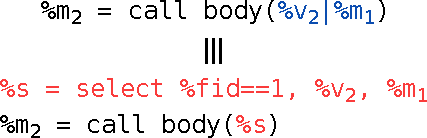
\includegraphics[scale=0.7]{src/merge-operation/figs/operand-select.pdf}
  \caption{Operand selection for the \texttt{call} instruction in \texttt{L\textsubscript{4}}
             from Figure~\ref{fig:code-gen-cfg}. Mismatching operands chosen
             with a \texttt{select} instruction on the function identifier.}
  \label{fig:operand-select}
\end{figure}

Whenever the corresponding operands of merged instructions are different, we
need a way to select the correct operand based on the function identifier.
Section~\ref{sec:label-select} describes how we perform label selection.
In all other cases, we simply use a \textit{select} instruction, as shown in
Figure~\ref{fig:operand-select}.

\begin{figure}[t]
  \centering
  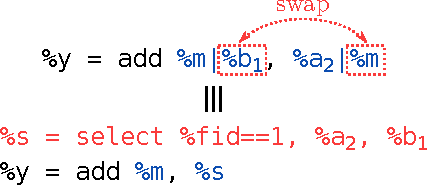
\includegraphics[scale=0.7]{src/merge-operation/figs/operand-select-reorder.pdf}
    \caption{Optimizing operand assignment for commutative instructions.
             Example of a merged \texttt{add} instruction that can have its
             operands reordered to allow merging the two uses of \texttt{\%m},
             avoiding a \textit{select} instruction.}
  \label{fig:operand-select-reorder}
\end{figure}

When assigning operands to commutative instructions, we also perform operand
reordering to maximize the number of matching operands and reduce the need for
\textit{select} instructions.
Figure~\ref{fig:operand-select-reorder} shows an example of a commutative instruction
where an operand selection can be avoided by reordering operands.
%This property of commutative operations has been exploited before by other
%optimizations~\cite{porpodas18a,porpodas19,rocha19}.

\subsubsection{Label Selection} \label{sec:label-select}

In LLVM, labels are used exclusively to represent control flow.
More specifically, label operands are used by terminator instructions, where
they specify the destination basic block of a control flow transfer, or
to represent incoming control flow in a \textit{phi-node} instruction.

Whenever assigning the operands of a merged terminator instruction, if there is
a label mismatch between the two input functions, we need a way to select
between the two labels depending on the executed function.
We do so by creating a new basic block with a conditional branch on the function
identifier to each one of the mapped labels. Then we use the new block's label as
the operand of the merged terminator instruction.
Figure~\ref{fig:label-select} illustrates a CFG that handles label selection for
a merged terminator instruction.

\begin{figure}[t]
  \centering
  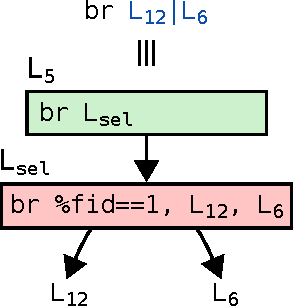
\includegraphics[scale=0.65]{src/merge-operation/figs/label-select.pdf}
  \caption{Label selection for mismatched terminator instruction operands
	\texttt{L\textsubscript{f1}} and \texttt{L\textsubscript{f2}} corresponding
	to labels of two different basic blocks. We handle control flow in a new
	basic block, \texttt{L\textsubscript{sel}} with a conditional branch on the
	function identifier targeting the two labels. We use the label of the new
	block as the merged terminator operand.}
  \label{fig:label-select}
\end{figure}

\subsubsection{Landing Blocks}

Most modern compilers, including GCC and LLVM, implement the zero-cost Itanium ABI for exception handling~\cite{dinechin00}, which is known
as the \textit{landing-pad} model. This model has two main components: $(1)$ invoke instructions that have two successors, one that
continues when the call succeeds as per normal, and another, usually called the \textit{landing pad}, in case the call raises an exception,
either by a throw or the unwinding of a throw; $(2)$ landing-pad instructions that encode which action is taken when an exception is
raised. A landing pad must be the immediate successor of an invoke instruction in its unwinding path. The code generator must ensure that
this model is preserved.

Our new code generator delays the creation of landing-pad instruction until
the phase of operand assignment.
Once we have concluded the remapping of all label operands of an invoke instruction,
regardless of whether they are merged or non-merged code, we create an
intermediate basic block with the appropriate landing-pad instruction.
Then we assign the label of this landing block as the operand of
the invoke instruction, as shown in Figure~\ref{fig:landingpad}.

\begin{figure}[t!]
  \centering
  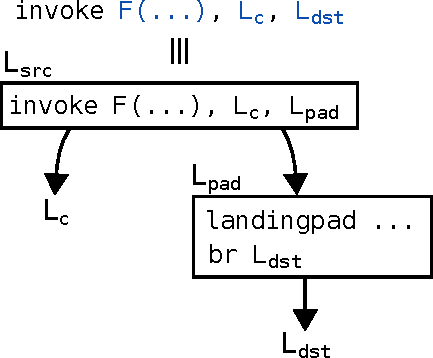
\includegraphics[scale=0.65]{src/merge-operation/figs/landingpad.pdf}
  \caption{Landing blocks are added after operand assignment and
	are assigned to invoke instructions as operands.}
  %\fixme{PP: not sure whether this plot is interesting.}
  \label{fig:landingpad}
\end{figure}

\subsubsection{Phi-Node's Incoming Values} \label{sec:phi-in-vals}

There are two distinct cases for \textit{phi-nodes}: being associated with a
matching or with a non-matching label. In both cases, \textit{phi-nodes} are
only copied from their input functions and they are not merged. So each
\textit{phi-node} in the merged function should capture the incoming flows
present in the corresponding \textit{phi-node} of their input function. For
matching labels, each \textit{phi-node} in the merged function will have
additional incoming flows specific to the \textit{other} input function but
these flows should have undefined values.

To assign the incoming values of a \textit{phi-node}, {\ProjName} iterates over
all predecessors of its parent basic block and uses the \textit{block mapping}
to discover each predecessor's corresponding basic block in the input function.
If such a basic block is found, then
{\ProjName} obtains the incoming value associated with that predecessor from the \textit{value mapping}.
Otherwise, an undefined value, which by construction should never be actually used,
is associated with that predecessor.

\subsection{Preserving the Dominance Property} \label{sec:ssa-fix}
%
%After code generation, {\ProjName} ends up with a code that violates the
%\textit{dominance property} of the SSA form.
The code transformation process described so far could violate the \textit{dominance property} of the SSA form. This property states that
each use of a value must be dominated by its definition. For example, an instruction (or basic block) dominates another if and only if
every path from the entry of the function to the latter goes through the former. Figure~\ref{fig:phi-placement-1} gives one example
extracted from Figure~\ref{fig:code-gen-cfg} where the the dominance property is violated during code transformation.

\begin{figure}[t]
  \centering
  \begin{subfigure}{.5\textwidth}
    \center
    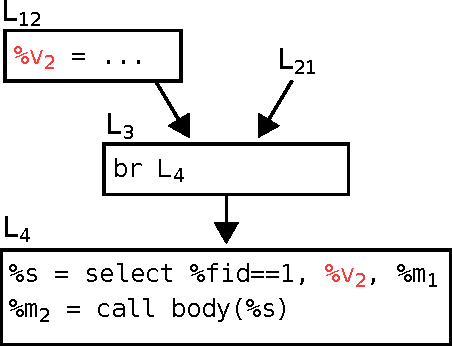
\includegraphics[scale=0.65]{src/merge-operation/figs/phi-placement-1}
    \caption{Example where the dominance property is violated.}
    \label{fig:phi-placement-1}
  \end{subfigure}
  \\
  \begin{subfigure}{.5\textwidth}
    \center
    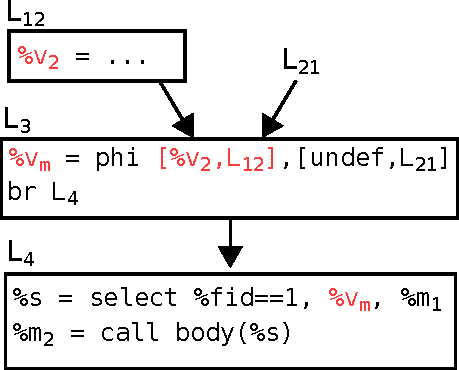
\includegraphics[scale=0.65]{src/merge-operation/figs/phi-placement-2}
    \caption{The dominance property is restored by placing phi-nodes where needed.}
    \label{fig:phi-placement-2}
  \end{subfigure}
  \caption{Example of how {\ProjName} uses the standard SSA construction algorithm
           to guarantee the dominance property of the SSA form.}
  \label{fig:phi-placement}
\end{figure}


%The dominance property states that each use of a value must be dominated by its definition. An instruction (or basic block) dominates
%another if and only if every path from the entry of the function to the latter goes through the former. Figure~\ref{fig:phi-placement-1}
%shows one small example extracted from Figure~\ref{fig:code-gen-cfg} that illustrates a violation of the dominance property. {\ProjName}
%restores this property by first adding a \textit{pseudo-definition} at the entry block of the function where names are defined and
%initialized with an \textit{undefined} value. This guarantees that every register name will be defined on basic blocks from both functions.
%Then, {\ProjName} applies the standard SSA construction algorithm~\cite{cytron89,cytron91}, which guarantees both the dominance and the
%single-reaching definition properties of the SSA form. Figure~\ref{fig:phi-placement-2} shows the resulting code.




{\ProjName} is designed to preserve the dominance property to conform with the SSA form.
It achieves this using a two-step approach.
It first adds a \textit{pseudo-definition} at the entry block of the function where names are defined and initialized with an
\textit{undefined} value.
This guarantees that every register name will be defined on basic blocks from both functions.
Then, {\ProjName} applies the standard SSA construction algorithm~\cite{cytron89,cytron91}, which guarantees both the dominance and the
single-reaching definition properties of the SSA form.
We note that our implementation uses the standard SSA construction algorithm provided by LLVM for register promotion.
This algorithm guarantees that names have a single definition by placing extra phi-nodes where needed so that instructions can be renamed appropriately.
Figure~\ref{fig:phi-placement-2} shows how the property violation in Figure~\ref{fig:phi-placement-1} can be corrected using this strategy.

%Formally, this algorithm can be described as follows.
%Given a set of definitions to the same name, the placement of phi-nodes consists of computing its \textit{iterated dominance frontier}, as define below:

%\begin{definition}[Dominance Frontier]
%The \textit{dominance frontier} of a node $n$, $DF(n)$, is the set of all nodes $n'$
%such that $n$ dominates an \textit{immediate} predecessor of $n'$ but does not \textit{strictly} dominate $n'$.
%This definition also extends to sets of nodes.
%The \textit{dominance frontier} of a set of nodes $S$ is the union of each \textit{dominance frontier},
%i.e., $DF(S) = \bigcup_{n\in S}DF(n)$.
%\end{definition}

%\begin{definition}[Iterated Dominance Frontier]
%The \textit{iterated dominance frontier} of a set of nodes $S$ is the limit $DF^+_{i\to\infty}(S)$ of the recurrence equation below:
%\begin{align*}
%DF^+_1(S) &= DF(S) \\
%DF^+_{i+1}(S) &= DF(S\cup DF^+_i(S))
%\end{align*}
%\end{definition}

%Given a register name $v$, phi-nodes are placed in all basic blocks from set $DF^+(Defs(n))$, where $Defs(v)$ is the set of all basic
%blocks, which contains a definition of $v$. For the example shown in Figure~\ref{fig:phi-placement}, we have
%$Defs(\texttt{\%v\textsubscript{2}}) = \{ \texttt{L\textsubscript{12}}, \texttt{L\textsubscript{1}} \}$, where the entry block
%\texttt{L\textsubscript{1}} contains the \textit{pseudo-definition}.

%%%
%%%Although this is enough to guarantee the correctness of the SSA form,
%%%there are still optimization opportunities that can be explored by {\ProjName}.
%%%We discuss these opportunities for optimization in the next section.

\subsection{Phi-Node Coalescing} \label{sec:pncoalescing}

The approach described in Section~\ref{sec:ssa-fix} guarantees the correctness of the SSA form but generates extra
phi-nodes and registers which increase register pressure and might lead to more \textit{spill code}. In this section, we describe a novel optimization technique, \textit{phi-node coalescing}, that {\ProjName} uses to lower register pressure.

%The approach described in Section~\ref{sec:ssa-fix} guarantees the correctness of the SSA form but leaves room for improvement.
%In this section, we describe \textit{phi-node coalescing}, a novel optimization technique employed by {\ProjName} to lower the register
%pressure on the final merged code by reducing the number of phi-nodes required.
%This reduces code size of the merged function since a lower register pressure allows the register allocator to produce fewer \textit{spill code}.

Figure~\ref{fig:phi-coalescing-select} illustrates such an optimization opportunity. {\ProjName} is merging an instruction with different arguments,
so it needs to select the right one based on the function identifier. The two arguments though, \texttt{v} and \texttt{x}, have \textit{disjoint definitions},
i.e. they have non-merged definitions from different input functions. Using the standard SSA construction algorithm would result in
the sub-optimal code shown in Figure~\ref{fig:phi-coalescing-select-1}. This code inserts two trivial phi-nodes to select, again, \texttt{v} or \texttt{x}
based on the executed function. {\ProjName} optimizes this code by coalescing both phi-nodes into a single one and removing the
selection statement. As shown in Figure~\ref{fig:phi-coalescing-select-2}, the optimized version has a smaller number of instructions and
phi-nodes.


%This example contains a pair of \textit{disjoint
%definitions} \texttt{v} and \texttt{x}, i.e. two non-merged definitions that came originally from different input functions. This pair of
%disjoint definitions is used via a selection in a merged instruction. Simply using the standard SSA construction algorithm would result in
%the sub-optimal code shown in Figure~\ref{fig:phi-coalescing-select-1}. This code has two trivial phi-nodes, one for the definition in each
%function, and a final selection. {\ProjName} further optimizes this code by coalescing both phi-nodes into a single one, removing the
%selection statement. As shown in Figure~\ref{fig:phi-coalescing-select-2}, the optimized version has a smaller number of instructions and
%phi-nodes.

\begin{figure}[t]
  \centering
  \begin{subfigure}{.5\textwidth}
    \center
    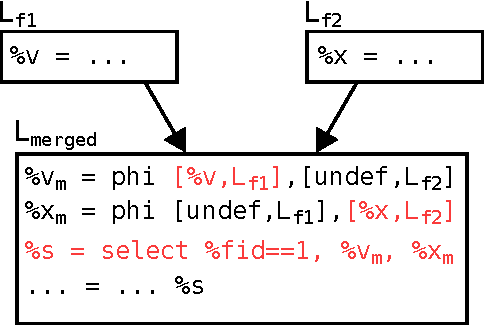
\includegraphics[scale=0.65]{src/merge-operation/figs/phi-coalescing-select-1}
    \caption{Phi-node placement without coalescing.}
    \label{fig:phi-coalescing-select-1}
  \end{subfigure}
  \\
  \begin{subfigure}{.5\textwidth}
    \center
    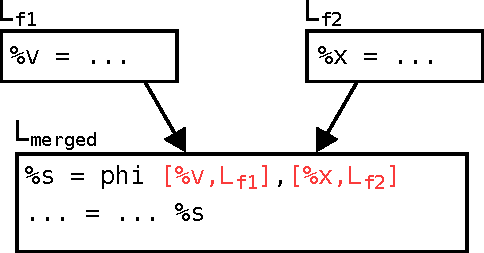
\includegraphics[scale=0.65]{src/merge-operation/figs/phi-coalescing-select-2}
    \caption{Phi-node placement with coalescing.}
    \label{fig:phi-coalescing-select-2}
  \end{subfigure}
  \caption{Phi-node coalescing reduces the number of phi-nodes and selections.}
  \label{fig:phi-coalescing-select}
\end{figure}

\begin{figure}[h]
  \centering
  \begin{subfigure}{.5\textwidth}
    \center
    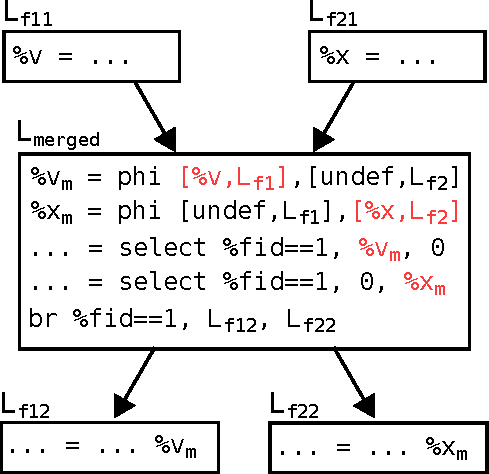
\includegraphics[scale=0.65]{src/merge-operation/figs/phi-coalescing-gen-1}
    \caption{Phi-node placement without coalescing.}
    \label{fig:phi-coalescing-gen-1}
  \end{subfigure}
  \\
  \begin{subfigure}{.5\textwidth}
    \center
    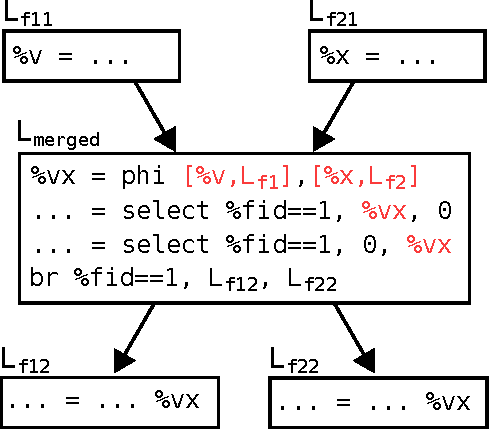
\includegraphics[scale=0.65]{src/merge-operation/figs/phi-coalescing-gen-2}
    \caption{Phi-node placement with coalescing.}
    \label{fig:phi-coalescing-gen-2}
  \end{subfigure}
  \caption{Reducing the number of phi-nodes by coalescing disjoint definitions with no user instructions
in common.}
  \label{fig:phi-coalescing-gen}
\end{figure}

This transformation is valid because a value definition that
is exclusive to a function will never be used when executing
the other function.
Figure~\ref{fig:phi-coalescing-gen} shows another example
illustrating that even disjoint definitions that have no user instructions
in common can be coalesced, reducing the number of phi-nodes.

Since {\ProjName} is aware of which basic blocks are exclusive to each function, it can choose a pair of disjoint definitions for
coalescing. Given a pair of disjoint definitions, {\ProjName} assigns the same name for both of them before applying the SSA
reconstruction. {\ProjName} coalesces the set of definitions that violate the dominance property. Two definitions can be paired for
coalescing if they are disjoint and have the same type. The optimization pairs disjoint definitions that maximize their live range overlap
since the goal is to avoid having register names live longer than they should, reducing register pressure.

Formally, the heuristic implemented in our phi-node coalescing can be described as follows:
Given a set $S_1\times S_2$ of disjoint definitions that violate the dominance property,
the optimization chooses pairs $(d_1,d_2)\in S_1\times S_2$ that maximize the intersection $U\!B(d_1)\cap U\!B(d_2)$,
where $U\!B(d)$ is the set \text{$\{ Block(u) : u\in Users(d) \}$}.

Phi-node coalescing allows {\ProjName} to produce smaller merged functions and reduce code size.
Consequently, it also enables more functions to be profitably merged.


\chapter{Function Merging Optimisation}

\section{Profitability Cost Model}\label{sec:profit-model}

After generating the code of the merged function, we need to estimate the
code-size benefit of replacing the original pair of functions by the new merged
function.
In order to estimate the code-size benefit, we first compute the code-size cost
for each instruction in all three functions.
In addition to measuring the difference in size of the merged function, we also
need to take into account all extra costs involved:
$(1)$ for the cases where we need to keep the original functions with a call to
the merged function;
and $(2)$ for the cases where we update the call graph, there might be an extra
cost with a call to the merged function due to the increased number of arguments.

Let $c(f)$ be the code-size cost of a given function $f$, and
$\delta(f_i, f_j)$ represent the extra costs involved when replacing or
updating function $f_i$ with the function $f_j$.
Therefore, given a pair of functions $\{f_1,f_2\}$ and the merged function
$f_{1,2}$, we want to maximise the profit defined as:
\[
  \Delta(\{f_1,f_2\},f_{1,2}) = (c(f_1)+c(f_2)) - (c(f_{1,2}) + \varepsilon)
\]
where $\varepsilon = \delta(f_1, f_{1,2}) + \delta(f_2, f_{1,2})$.
We consider that the merge operation is profitable if $\Delta(\{f_1,f_2\},f_{1,2})>0$.

However, because we are operating on the IR level, one IR instruction does not
necessarily translate to one machine instruction.
Because of that, the profitability is measured with the help of the compiler's
target-specific cost model.
The actual cost of each instruction comes from querying this compiler's built-in
cost model, which provides a target-dependent cost estimation that approximates
the code-size cost of an IR instruction when lowered to machine instructions.
Our implementation makes use of the code-size costs provided by LLVM's
target-transformation interface (TTI), which is widely used in the decision
%making by most of the LLVM's optimisations.
making of most optimisations~\cite{porpodas18b,pohl18}.


\section{Exhaustive Search}


\section{Focusing on Profitable Functions}
\label{sec:framework}

%In this section, we describe our implementation of the function merging
%optimisation, which combines the proposed function-merging technique with an
%efficient exploration infrastructure.

%In this section, we describe our exploration infrastructure for the
%function merging optimisation.
Although the proposed technique is able to merge any two functions, it is not always profitable to merge them. In fact, as it is only
profitable to merge functions that are sufficiently similar, for most pairs of functions, merging them increases code size.
In this section, we introduce our framework for efficiently exploring the
optimisation space, focusing on pairs of functions that are profitable to merge. 

%Therefore,
%the main goal of our exploration infrastructure is to efficiently find pairs of functions that are profitable to merge.
%%
%As described in Section~\ref{sec:background}, LLVM's existing function merging
%optimisation, due to its hard restriction of only merging identical functions,
%is able to  efficiently explore which functions to merge by computing a hash
%of the functions.
%If two functions have the same hash, they are very likely to be identical.
%Moreover, merging identical functions is always profitable.
%For the proposed function-merging technique, on the other hand, because it is
%able to merge any pair of functions, we have a much larger exploration space and
%also a more challenging decision problem.

%\subsection{Ranking Infrastructure}

For every function, ideally, we would like to try to merge it with all other functions and choose the pair that maximises the reduction in
code size. However, this quadratic exploration over all pairs of functions results in prohibitively expensive compilation
overhead. In order to avoid the quadratic exploration of all possible merges, we propose the exploration framework shown in
Figure~\ref{fig:func-merge-opt-arch} for our optimisation.
\begin{figure}[t!]
  \centering
  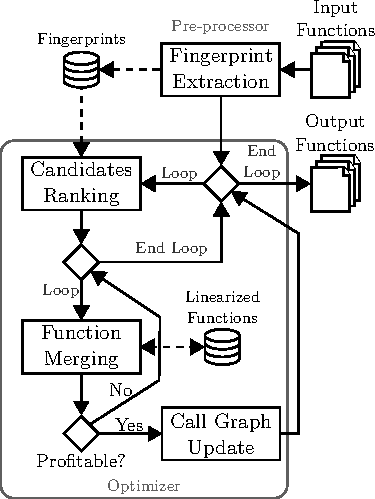
\includegraphics[width=0.7\linewidth]{src/merging-optimisation/figs/func-merge-opt-arch.pdf}
  \caption{Overview of our exploration framework.}
  \label{fig:func-merge-opt-arch}
\end{figure}

The proposed framework is based on a light-weight ranking infrastructure that uses a \textit{fingerprint} of the functions to evaluate
their similarity. It starts by precomputing and caching fingerprints for all functions. The purpose of fingerprints is to make it easy
to discard unpromising pairs of functions so that we perform the more expensive evaluation only on the most promising pairs.
To this end, the fingerprint consists of: $(1)$ a map of instruction opcodes to their frequency in the function; $(2)$ the set of types
manipulated by the function. While functions can have several thousands of instructions, an IR usually has just a few tens of opcodes,
e.g., the LLVM IR has only about 64 different opcodes. This means that the fingerprint needs to store just a small integer array of the
opcode frequencies and a set of types, which allows for an efficient similarity comparison.

By comparing the opcode frequencies of two functions, we are able to estimate
the best case merge, which would happen if all instructions with the same opcode could match.
This is a very optimistic estimation. It would be possible only if instruction types and order
did not matter. We refine it further by estimating another best case merge, this time based
on type frequencies, which would happen if all instructions with the same data type could match.


%This assumption provides an upper bound on the actual number of matches, since
%it may be affected by the instruction types and the order they appear in the
%linearised functions.
%As a way to refine this estimate, we weight this upper bound by the Jaccard
%similarity coefficient~\cite{jaccard} of the sets of types, i.e., a
%type-similarity ratio between the two functions.
%Formally, let $T_1$ and $T_2$ be the set of types of the functions $f_1$ and
%$f_2$, respectively.
%In order to refine this upper-bound estimate, we also compare the type frequencies
%of the two functions, this time assuming that all instructions with the same
%data type would always result in a match.
Therefore, the upper-bound reduction, computed as a ratio, can be generally defined as
%\[
%   U\!B(f_1,f_2) = \frac{\sum\limits_{op \in Ops} \min\{freq(op,f_1),freq(op,f_2)\}}{\sum\limits_{op \in Ops} freq(op,f_1)+freq(op,f_2)}
%\]
\[
   U\!B(f_1,f_2, K) = \frac{\sum\limits_{k \in K} \min\{freq(k,f_1),freq(k,f_2)\}}{\sum\limits_{k \in K} freq(k,f_1)+freq(k,f_2)}
\]
where $U\!B(f_1,f_2, Opcodes)$ computes the opcode-based upper bound and
$U\!B(f_1,f_2, Types)$ computes the type-based upper bound.
The final estimate selects the minimum upper bound between the two, i.e.,
\[
%     s(f_1,f_2) = U\!B(f_1,f_2) \frac{|T_1 \cap T_2|}{|T_1 \cup T_2|}.
     s(f_1,f_2) = \min\{U\!B(f_1,f_2, Opcodes), U\!B(f_1,f_2, Types)\}
\]
This estimate results in a value in the range $[0,0.5]$,
which encodes a description that favors maximizing both the opcode and type
similarities, while also minimizing their respective differences.
Identical functions will always result in the maximum value of $0.5$.

For each function $f_1$, we use a priority queue to rank the topmost
similar candidates based on their similarity, defined by $s(f_1,f_2)$, for all
other functions $f_2$.
We use an exploration threshold to limit how many top candidates we will
evaluate for any given function.
We then perform this candidate exploration in a greedy fashion, terminating after
finding the first candidate that results in a profitable merge and committing that
merge operation.

\begin{figure}[t!]
  \centering
  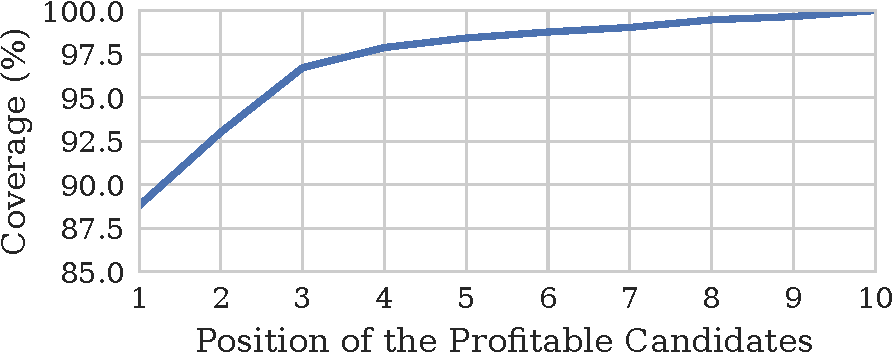
\includegraphics[width=0.8\linewidth]{src/merging-optimisation/figs/average-cdf-exploration-threshold.pdf}
  \caption{Average CDF for the position of the profitable candidate and the percentage of merged operations covered.
           %Average CDF for the exploration threshold and the percentage of merged operations covered.
           89\% of the merge operations happen with the topmost candidate.}
           %A merge operation happens with the topmost candidate in about 89\% of the cases.}
  \label{fig:average-cdf-exploration-threshold}
\end{figure}

Ideally, profitable candidates will be as close to the top of the rank as
possible.
Figure~\ref{fig:average-cdf-exploration-threshold} shows the cumulative
distribution of the position of the profitable candidates in a top 10 rank.
It shows that about 89\% of the merge operations occurred with the topmost
candidate, while the top 5 cover over 98\% of the profitable candidates.
These results suggest that fingerprint similarity is able to
accurately capture the real function similarity, while reducing the exploration
cost by orders of magnitudes, depending on the actual number and size of
the functions.

When a profitable candidate is found, we first replace the body of the two
original functions to a single call to the merged function.
Afterwards, if the original functions can be completely removed, we update the
call graph, replacing the calls to the original functions by calls to the
merged function.
Finally, the new function is added to the optimisation working list.
Because of this feedback loop, merge operations can also be performed on
functions that resulted from previous merge operations.

\subsection{Link-Time Optimisation}

There are different ways of applying this optimisation, with different trade-offs.
We can apply our optimisation on a per compilation-unit basis, which usually
results in lower compilation-time overheads because only a small part of the
whole program is being considered at each moment.
However, this also limits the optimisation opportunities, since only pairs of
functions within the same translation unit would be merged.

On the other hand, our optimisation can also be applied in the whole program,
for example, during link-time optimisation (LTO).
Optimizing the whole program is beneficial for the simple fact that the
optimisation will have more functions at its disposal.
It allows us to merge functions across modules.

\begin{figure}[h]
  \centering
  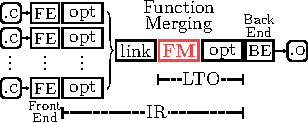
\includegraphics[width=0.7\linewidth]{src/merging-optimisation/figs/opt-pipeline.pdf}
  \caption{In our experiments we use a compilation pipeline with a monolithic link-time optimisation (LTO).}
  \label{fig:opt-pipeline}
\end{figure}


In addition to the benefit of being able to merge more functions, when optimizing
the whole program, we can also be more aggressive when removing the original functions,
since we know that there will be no external reference to them.
However, if the optimisation is applied per translation unit, then extra
conditions must be guaranteed, e.g., the function must be explicitly defined
as internal or private to the translation unit.


\chapter{Reducing Runtime Overhead}

The identical function merging has no runtime penalty since it only alias two identical functions, removing one of the copies.
However, merging partially similar functions may introduce runtime overheads in a given execution path.

Figure~\ref{fig:partially-merged-blocks} shows an example of how function merging may introduce runtime overheads when merging two partially equivalent basic blocks.
The two basic blocks involved in this merge operation were extracted from the \texttt{462.libquantum} benchmark.
This example illustrates two different types of overheads that may be introduced during function merging:
$(i)$ the insertion of value selections;
$(ii)$ the insertion of branches to diverge to mismatching code or converge to matching code.


\begin{figure}[t]
  \centering
  \begin{subfigure}{\textwidth}
    \center
    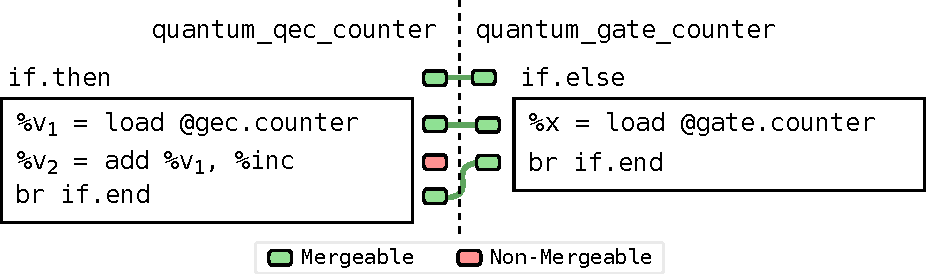
\includegraphics[scale=0.8]{src/runtime-overhead/figs/partially-merged-blocks-alignment}
    \caption{Pair of aligned basic blocks extracted from two larger functions in the \texttt{462.libquantum} benchmark.}
    \label{fig:partially-merged-blocks-alignment}
  \end{subfigure}
  \\
  \begin{subfigure}{\textwidth}
    \center
    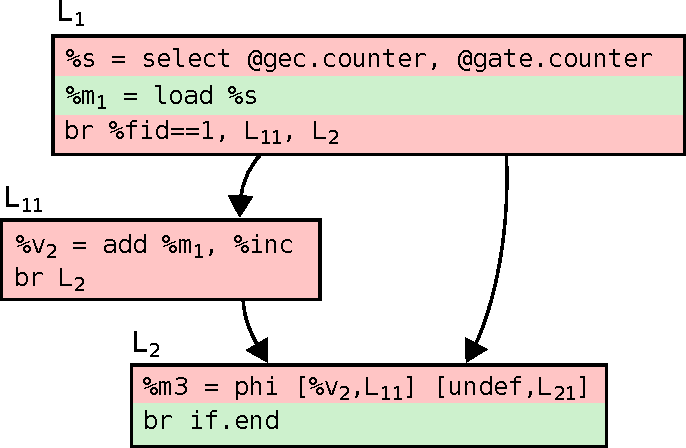
\includegraphics[scale=0.8]{src/runtime-overhead/figs/partially-merged-blocks-codegen}
    \caption{Merged code generated for the pair of aligned basic blocks.}
    \label{fig:partially-merged-blocks-codegen}
  \end{subfigure}
  \caption{Example of how function merging may introduce runtime overheads. }
  \label{fig:partially-merged-blocks}
\end{figure}

\section{Conservative Function Merging}\label{sec:conservative-fm}

In this section, we propose a conservative function merging approach that aims at minimal runtime overhead in the absence of profiling information.
The function merging approach described in Chapter~\ref{chap:fm-operation} is capable of partially merging basic blocks, inserting branches between instructions to split matching from non-matching code.
In order to minimise runtime overheads on possibly hot basic blocks, our conservative approach consider only merging whole basic blocks.

\section{Profile-Guided Function Merging}


\chapter{Conclusion} \label{chp:conclusion}

This thesis presents a novel compiler optimisation for reducing code size by merging functions.
Chapter~\ref{chp:fm-operation} describes our novel approach, based on sequence alignment, for merging any two functions.
Chapter~\ref{chp:opt-strategy} describes how our function merging technique can be combined with a optimisation strategy in order to search for profitable functions to merge, which includes a profitability cost model and a ranking of candidate functions.

This chapter is structured as follows:
Section~\ref{sec:conclusion:contribution} summarises the main contributions of this thesis,
%Section 7.2 presents a critical analysis of this work,
Section~\ref{sec:conclusion:futurework} describes future research directions,
and finally Section~\ref{sec:conclusion:summary}  provides concluding remarks.


% We have presented {\ProjName}, a novel compiler-based function merging technique with full support for the SSA form.
% Unlike the previous state-of-the-art, which has to apply register demotion to eliminate the commonly used \textit{phi-nodes} in SSA,
% {\ProjName} directly processes \textit{phi-nodes} using a more powerful code generator.
% As a result, {\ProjName} avoids the code bloating problem introduced by register demotion and
% increases the chances of generating profitable merged functions. We have implemented {\ProjName} in LLVM and evaluated it on the SPEC CPU2006
% and CPU2017 benchmark suites. {\ProjName} delivers on average 9.5\% code reduction for the lowest exploration threshold. Compared to the previous
% function merging state-of-the-art, {\ProjName} achieves $2\times$ more reduction on binary size with 3$\times$ less compile-time overhead and less than half the amount of memory required by it.

% We proposed a novel function merging approach based on sequence alignment, called FMSA. This was the first technique capable of merging any two functions, if deemed profitable, achieving up to 30\% of code-size reduction on SPEC 2006, about twice as much as the past state of the art.
% Although this technique offers significant improvements over previous ones, there are still many limitations and missed opportunities that prevent us from achieving all the available code compression.
% We need to improve the code generator, exploit code reordering, work at different scopes, scale to huge programs, avoid runtime slowdowns, work on JITs, and adopt machine learned heuristics.
% %To address these missed opportunities,
% %We plan to create a better code generator, a new approach that handles code reordering and merges code across different scopes, more accurate cost models
% %, with a better ranking mechanism and code aligner powered by deep learning.
% This will result in smaller programs without runtime or compile time overheads.

\section{Contribution} \label{sec:conclusion:contribution}

This thesis presents a novel function merging technique alongside an optimisation strategy.
Our novel technique uses sequence alignment algorithms from bioinformatics in order to identify the similarity between functions being merged.
The proposed optimisation is very effective at reducing code size by merging arbitrary functions.
Our approach does not suffer from any of the major limitations of existing solutions, outperforming them by more than 2.4$\times$.
We also proposed a ranking-based exploration mechanism to focus the optimization on promising pairs of functions.
Ranking reduces the compilation-time overhead by orders of magnitude compared to an exhaustive quadratic exploration. 
With this framework, our optimization is able to reduce code size by up to 25\%, with an overall average of about 6\%, while introducing an average compilation-time overhead of only 15\%.
Coupled with profiling information, our optimization introduces no statistically significant impact on performance.

\section{Future Work} \label{sec:conclusion:futurework}

For future work, we plan to focus on improving the ranking mechanism to reduce compilation time.
In order to avoid code size degradation, we also plan to improve the compiler's built-in static cost model for code size estimation.
We also plan to work on the linearisation of the candidate functions, allowing instruction reordering to maximize the number of matches between the functions.
Finally, we also plan to incorporate instruction reordering into function merging to maximize the number of matches between the functions regardless of the original code layout.
One can also investigate the application of phi-node coalescing outside function merging.
We envisage further improvements can be achieved by integrating the function-merging optimization to a summary-based  link-time optimization framework, such as ThinLTO in LLVM.
As a future work, we can also analyze the interaction between function merging and other optimizations such as inlining, outlining, and code splitting.

\subsection{Better Code Generator}

%FMSA's code generator is responsible for producing the actual merged functions from the aligned sequences.
%In its original version, FMSA has many artificial limitations in order to simplify its code generator.
%Preliminary results show that the code generator can be significantly improved, enabling far more code compression while reducing compilation time overhead.
%For this project, we plan to develop a new code generator that is capable of appropriately handling $\phi$-nodes, variable length arguments, calling convention, and exploiting target specific instructions to better compress code.
%There are still many opportunities to optimize operand selection and branch instructions that result from merging code. 

In order to better compress code, one can improve the code generator, optimising the parameters used as function identifiers based on calling conventions, exploit target specific instructions, and optimize operand selection and branch instructions that result from merging code.
There are also many missing features in the code generator that are important for its application in the industry.
For example, a new code generator could also be able to appropriately handle variable length arguments, and debug information.
When merging functions, having an optimised code generator is as important as optimally identifying which instructions to merge.
%In the industry, it is also crucial that we appropriately handle debug information when generating code. %link with: \phi$-nodes, variable length arguments
%Appropriately generating code with debug information is crucial for its application in the industry.

\subsection{Handling Code Reordering}

All existing function merging techniques rely on the order in which instructions appear inside the basic blocks and their arrangement,
failing to profitably merge equivalent functions when confronted even with the smallest variations on the ordering of instructions and basic blocks.
Figure~\ref{fig:code-reordering} shows an example of two functions that all existing techniques fail to merge even though they are obviously identical.
Our current technique produces the merged function shown in Figure~\ref{fig:merged-code-reordering}, which is considered unprofitable as it is unable to reduce code size.
Note that all indexing computation is duplicated, including the increment operation, resulting in a merged function that is unnecessarily bigger than the two original functions together.
We need more powerful graph, rather than sequence, alignment techniques to better identify and merge differently ordered but semantically equivalent code.

\begin{figure}[h]
 \centering
 \begin{subfigure}{.5\textwidth}
         \centering
         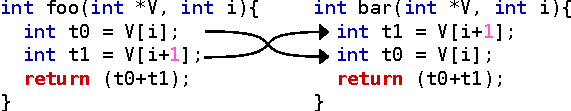
\includegraphics[scale=0.85]{src/conclusion/figs/motivation-1-code.pdf}
         \vspace{1ex}
         \caption{Two equivalent functions.}
         \label{fig:code-reordering}
 \end{subfigure}\begin{subfigure}{.5\textwidth}
         \centering
         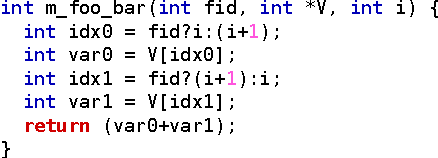
\includegraphics[scale=0.85]{src/conclusion/figs/motivation-1-merged-code.pdf}
         \caption{Merged function currently produced by FMSA.}
         \label{fig:merged-code-reordering}
 \end{subfigure}
    \vspace{-2ex}
    \caption{Example of how even trivial reordering is poorly handled by the existing solutions.}
    \label{fig:code-reordering-example}
\end{figure}

\subsection{Merging Across All Scopes}

Existing techniques are limited to one particular scope.
While function merging is applied only to whole functions,
function outlining is commonly applied at the basic block level.
%In one end we have an optimization such as the function outlining which is capable of merging or extracting equivalent basic blocks, in the other end we have function merging capable of merging whole functions.
However, equivalent code can be found within or across functions, which themselves may reside in the same source file or be spread across multiple source files.
Therefore, we need to develop a novel unified optimization capable of merging semantically equivalent code that can span anything between a single basic block up to a whole function.
This unification has the extra benefit of also addressing the phase ordering problem by coordinating the merge operations on different scopes.

\subsection{Scaling for Large Programs}

Although our optimisation achieves very good results in terms of code compression, it is still unable to handle large programs in a real scenario.
Its time complexity and memory usage requirements would prevent it from optimizing large programs such as web browsers, Clang/LLVM, and operating systems, as these programs tend to have many functions with several thousands of instructions.
Link-time optimization (LTO) makes this matter even worse by optimizing the code after the whole program has been linked into a single module, imposing a huge pressure on memory usage and compilation time.

%In this project, we will investigate this scalability issue.
%We plan to perform link-time optimization in an incremental fashion, such as using ThinLTO, which operates on individual translation units, reducing memory usage while also making it suitable for parallel and distributed compilation.
The optimization of different translation units can be distributed across different machines and merge operations locally performed in parallel.
In order for this to work, an important challenge that needs to be addressed concerns ranking and merging functions that reside in different translation units.
However, this is essential to enable the use of LTO on real programs while keeping the memory usage and compilation time acceptable.

\subsection{Powered by Deep Learning}

In order to reduce compilation time while also being effective, 
the ranking-based exploration mechanism tries to efficiently focus the search 
only to the most promising pairs of functions.
However, the existing solution is still very wasteful as most of the merged functions are
discarded by the profitability analysis.
Identifying what would be profitably merged is a very challenging task.

Given our group's expertise on the area, we plan to use solutions based on deep learning to efficiently predict which pairs of functions are most likely to be profitable to merge.
This approach has the potential to reduce compilation time even further while also improving the compression by finding profitable candidates that are currently missed.
Having accurate target-specific cost models is crucial for the effectiveness of the profitability analysis.
We plan to explore the use of machine learning techniques to develop more accurate cost models.

One can investigate the use of deep learning to align two functions and better identifying what can be merged.
Sequence alignment focusses only on maximizing the number of merged instructions,
without necessarily minimizing the number of operand selections or branches.
A smarter approach that understands how instructions interact with each other would be
very beneficial.


\subsection{Avoiding Performance Overheads}

For many real applications, it is desirable to achieve a good balance between code size and performance.
Preliminary results show that performance degradation can be completely avoided by using profiling to
guide the merging decisions.
One can avoid adding branches inside hot execution paths, therefore avoiding performance penalties.
Although hot code can be merged, it is important to minimize unnecessary branches when merging hot code.
We will develop a profile-guided optimization that automatically identify the best trade-off between code-size and performance.

\subsection{Less Memory Usage by JIT}

Ahead-of-time and just-in-time (JIT) compilation have completely different requirements.
Function merging can be used to reduce the amount of memory used by programs running on a JIT environment.
However, our solution must be adapted to the requirements that are specific to a JIT environment, as JIT compilers have the extra challenge of having to optimize the code as fast as possible.
This would require the development of completely new algorithms for ranking and aligning functions that are suitable for this application domain.
Another possibility is to exploit the fact multiple programs may be simultaneously running on the same JIT environment and merge code across different programs, reducing the overall memory usage.

\section{Summary} \label{sec:conclusion:summary}

%%%%%%%%
%% Any appendices should go here. The appendix files should look just like the
%% chapter files.
%\appendix
%\include{appendix1}
%% ... etc...

%% Choose your favourite bibliography style here.
%\bibliographystyle{apalike}
%\bibliographystyle{plainnat}
\bibliographystyle{plain}

%% If you want the bibliography single-spaced (which is allowed), uncomment
%% the next line.
% \singlespace

%% Specify the bibliography file. Default is thesis.bib.
\bibliography{
    bib/benchmarks.bib,
    bib/books.bib,
    bib/compilers.bib,
    bib/costmodel.bib,
    bib/func-merge.bib,
    bib/seqalign.bib
}

%% ... that's all, folks!
\end{document}
